\section{Swappable edges and their classification}

\subsection{Twisted Bruhat graphs}

The Bruhat order on the weight lattice $X$ is the order generated by the following relations

	
\begin{equation}\label{bruhatorder}s_\alpha^\vee(\lambda)< \lambda \iff \begin{cases}\langle \lambda,\beta^\vee\rangle > M &\text{if }M\geq 0,\\
\langle \lambda,\beta^\vee\rangle <  M&\text{if }M<0.\end{cases}\end{equation}
where $\alpha^\vee=M\delta+\beta^\vee$, with $\beta^\vee\in \Phi_+^\vee$ and $\lambda\in X$. The set of elements smaller that $\lambda$ in the Bruhat order, which we denote by $\{\leq \lambda\}$, can be characterized as
\begin{equation}\label{smallerthanlam}
    \{\leq \lambda\} =\Conv(W\cdot \lambda)\cap (\lambda+\bbZ\Phi)
\end{equation}
(see for example \cite[Chap. VIII, §7, exerc. 1]{Bou78}).

Let $\lambda\in X_+$. Let $\Gamma_\lambda$ denote the moment graph of the Schubert variety $\sch{\lambda}$. This is a directed labeled graph, also called the \emph{Bruhat graph} of $\lambda$. We recall  from \cite[\S 2.3]{Pat} the explicit description of $\Gamma_\lambda$.
The vertices of the graph $\Gamma_\lambda$ are all the weights in $\{\leq \lam\}$. We have an edge $\mu_1\raw \mu_2$ in $\Gamma_\lambda$ if and only if $\mu_2-\mu_1$ is a multiple of a root $\beta\in \Phi$ and $\mu_1\leq \mu_2$. In this case, the label of the edge $\mu_1\raw \mu_2$ is $m\delta-\beta^\vee$, where
\[m =-\frac{\langle \beta^\vee,\mu_1+\mu_2\rangle}{2}\] (cf. \cite[Lemma 2.6]{Pat}).  Notice that $s_{m\delta-\beta^\vee}(\mu_1)=\mu_2$. We denote by $E(\lambda)$ the set of edges in $\Gamma_\lam$.

Let $\Gamma_X$ denote the union of all the graphs $\Gamma_{\lambda}$, for $\lambda\in X_+$ (where $\Gamma_{\lambda}$ is regarded as a subgraph of $\Gamma_{\lambda'}$ if $\lambda\leq \lambda'$) and call it the Bruhat graph of $X$.





For $w\in \affW$ we denote by \[N(w):=\{\alpha \in \affPhi^\vee_+\mid w^{-1}(\alpha)\in \affPhi^\vee_-\}\] the set of inversions.
If $w=s_{i_1}\ldots s_{i_k}$ is a reduced expression for $w$ then \[N(w)=\{\alpha^\vee_{i_1},s_{i_1}(\alpha^\vee_{i_2}),\ldots,s_{i_1}s_{i_2}\ldots s_{i_{k-1}}(\alpha^\vee_{i_k})\}.\] 

We say that $w=s_1s_2\ldots s_k\ldots$ is a reduced infinite expression if for any $j$  the starting expression $w_j:=s_1s_2\ldots s_j$ is reduced.
If $w$ is a reduced infinite expression, let $N(w)=\bigcup_{j=1}^\infty N(w_j)$.


Consider $\undc = s_0s_2s_1s_2$. Then $y_\infty:=\undc \undc \undc\ldots$ is an infinite reduced expression.
Let $y_m$ be the element given by the first $m$ simple reflections in $y_{\infty}$.
We order the roots in $N(y_\infty)$ as follows:
\begin{multline}\label{reflectionorder}
\delta-\alpha_{21}^\vee<\delta-\alpha_{12}^\vee<2\delta-\alpha_{21}^\vee<  \delta -\alpha_{2}^\vee< 3\delta-\alpha_{21}^\vee<2\delta-\alpha_{12}^\vee< \\
\ldots<M\delta-\alpha_{12}^\vee<2M\delta-\alpha_{21}^\vee<M\delta-\alpha_{2}^\vee<(2M+1)\delta-\alpha_{21}^\vee<\ldots    
\end{multline}
so that the first $m$ roots in \eqref{reflectionorder} are precisely the elements of $N(y_m)$.

%We just write $\ell_m$ and $\leq_m$ for $\ell_{N(y_m)}$ and $\leq_{N(y_m)}$, the $y_m$-twisted length and the $y_m$-twisted Bruhat order on $\affW$.


	We define the \emph{$m$-twisted Bruhat order} $\leq_m$ of $\extW$ by setting 
	\[v\leq_m w\text{ if and only if }y_m^{-1}v\leq y_m^{-1}w,\]
	and the $m$-twisted length by $\ell_m(v):=\ell(y_m^{-1}v)$. 
Recall that $X\cong \extW/W$. Hence, the twisted Bruhat order on $\extW$ also induces a twisted Bruhat order on $X$. Concretely, this means that we regard $\lambda\in X$ as a right coset in $\extW$ and denote by $\lambda_m\in \extW$ the element of minimal $y_m$-twisted length in the coset $\lambda$. Then we set $\ell_m(\lambda):=\ell_m(\lambda_m)$ and $\mu\leq_m \lambda$ if $\lambda_m\leq_m \mu_m$.


	For every $m\in \bbZ_{\geq 0}$ we define $\Gamma_\lambda^m$, the $y_m$\emph{-twisted Bruhat graph of} $\lambda$, to be the directed labeled graph with the same vertices of $\Gamma_{\lambda}$ and where there is an edge $\mu\ra \lambda$ if there exists $\alpha^\vee\in \affPhi^\vee$ such that $s_{\alpha^\vee}(\mu)=\lambda$ and $\mu<_m \lambda$. Concretely, we can obtain $\Gamma_\lambda^m$ from $\Gamma_{\lambda}$ by inverting the orientation of all the arrows in $\Gamma_\lambda$ with label in $N(y_m)$.
	
	Since each graph $\Gamma_{\lambda}$ has only a finite number of edges, the twisted graphs $\Gamma_{\lambda}^m$ stabilize for $m$ big enough, so we can define $\Gamma_{\lambda}^\infty:=\Gamma_{\lambda}^m$ for $m\gg 0$. 

For $m\in \bbZ_{\geq 0} \cup \{\infty\}$, we define $\Gamma^m_X$ as the union of all the graphs $\Gamma^m_\lambda$, for $\lambda\in X_+$. The graph $\Gamma^m_X$ can be obtained from $\Gamma_X$ by inverting the orientation of all the arrows with label in $N(y_m)$.



\begin{definition} 
\label{twistedarrowslambdamu}
	For $\mu\leq \lambda$, we denote by $\Arr_m(\mu,\lam)$ the set of arrows pointing to $\mu$ in $\Gamma_m^\lambda$ and by $\ell_m(\mu,\lambda):=|\Arr_m(\mu,\lam)|$ the number of those arrows. 
	
	For $i \in \{1,2,21,12\}$ let $\Arr_m^{i}(\mu,\lam)$ be arrows pointing to $\mu$ in $\Gamma_m^\lambda$ of the form $\mu-k\alpha_i\raw \mu$ for $k\in \bbZ$. Let $\ell_m^i(\mu,\lam)=|\Arr_m^{i}(\mu,\lam)|$.
	
	Let $\Arr_\mu(\mu)$ be the set of arrows pointing to $\mu$ in $\Gamma_X^m$. For $i\in \{1,2,21,12\}$, the set $\Arr_m^i(\mu)$ is defined accordingly.
\end{definition}

Recall from \cite[Lemma 4.6]{Pat} that $|\Arr_m(\mu)|=\ell_m(\mu)$. We have 
\begin{equation}\label{ellsubdivided} \Arr_m(\mu,\lambda)=\bigcup_{i\in \{1,2,12,21\}}\Arr_m^i(\mu,\lambda)\quad\text{and}\quad
\ell_m(\mu,\lambda)=\sum_{i\in \{1,2,12,21\}} \ell_m^i(\mu,\lam)
 \end{equation}
 for any $\mu\leq \lambda$. Notice that, since there are no arrows in $N(y_\infty)$ of the form $M\delta-\alpha_1^\vee$, the set $\Arr_m^1(\mu,\lambda)$ does not depend on $m$, and does not depend on $\lambda$ as long as $\mu\leq \lambda$. If $\mu \leq \lambda$, for all $m$ by \eqref{bruhatorder} we have 
 \begin{align*}
 \Arr_m^1(\mu,\lambda)&=\{\mu - k\alpha_1\ra \mu \mid \mu-k\alpha_1\leq \mu\}\\
 &=\begin{cases}
 \{\mu - k\alpha_1\ra \mu \mid 0<k\leq \mu_1\}&\text{if }\mu_1\geq 0\\
 \{\mu - k\alpha_1\ra \mu \mid 0>k>\ \mu_1\}&\text{if }\mu_1< 0.
 \end{cases}
 \end{align*}
Hence, we have  \begin{equation}\label{ell1}\ell_m^1(\mu,\lam)=\begin{cases} \mu_1 &\text{if }\mu_1\geq 0\\
-\mu_1-1& \text{if }\mu_1<0.\end{cases}\end{equation}


\subsection{Swappable edges}

To pass from $\Gamma^m_\lambda$ to $\Gamma^{m+1}_\lambda$ (and from $\Gamma^m_X$ to $\Gamma^{m+1}_X)$ we need to invert the arrows with label $\alpha^\vee_{t_{m+1}}$, where $t_{m+1}$ is the reflection \begin{equation}\label{tm}t_{m+1}:=y_{m+1}y_m^{-1} =y_ms'_{m+1} y_m^{-1}.
\end{equation}
Here $s'_{m+1}$ denotes the $(m+1)$-th simple reflection in $y_\infty$.
Notice that $\{\alpha^\vee_{t_{m+1}}\}= N(y_{m+1})\setminus N(y_m)$.


If $\mu < t_{m+1}\mu$, then $\Arr_{m+1}(t_{m+1}\mu)\setminus \Arr_m(t_{m+1}\mu)=\{\mu\raw t_{m+1} \mu\}$ and $\Arr_{m}(\mu)$ is in bijection with $\Arr_{m}(t_{m+1}\mu)\setminus \{\mu\raw t_{m+1}\mu\}$ by \cite[Lemma 4.8]{Pat}. In particular, we have 
\begin{equation}\label{lmX}
\ell_m(\mu)=\ell_m(t_{m+1}\mu)-1.
\end{equation}



A remarkable property of the twisted Bruhat graphs in type $A$ (\cite[Prop. 4.14]{Pat}) is that the same is true if we restrict to $\Gamma_\lambda$, i.e. $\ell_m(\mu,\lambda)=\ell_m(t_{m+1}\mu,\lambda)-1$ if $\mu <t_{m+1}\mu \leq \lambda$. This implies that
$\ell_{m+1}(\mu,\lambda)=\ell_m(t_{m+1}\mu,\lambda)$ and $\ell_m(\mu,\lam)=\ell_{m+1}(t_{m+1}\mu,\lam)$. However, as we will see in \Cref{exampleswap}, this property does not hold in type $C_2$. The goal of this section is to classify the set of edges for which it holds.


\begin{definition}
\label{def:swappableedge}
	We say that an edge $\mu \raw t_{m+1}\mu$ in $\Gamma_{\lambda}$ is \emph{swappable} if 
 \begin{equation}\label{eqswapdef}
 \ell_m(\mu,\lambda)= \ell_m(t_{m+1}\mu,\lambda)-1.
 \end{equation}
 We also say that an edge is \emph{NS} if it is not swappable.
	We denote by $E^S(\lambda)$ and $E^N(\lambda)$ the sets of swappable and non-swappable edges in $\Gamma_\lambda$, respectively. 
\end{definition}


As it turns out, to determine if an edge is swappable or not, we have to solve an elementary geometric problem,  as the next example illustrates.

%We denote an element $\nu\in X$ as $\nu=(\nu_1,\nu_2)$, where
%$\nu_1:=\langle \nu,\alpha_1^\vee\rangle$ and $\nu_2:=\langle \nu,\alpha_2^\vee\rangle$ so that $\nu=\nu_1 \varpi_1 + \nu_2 \varpi_2 $. Note that this is not the same as the notation for the corresponding partition. %which would correspond to $(\nu_{1}+\nu_{2},\nu_{2})$.


\begin{example}\label{exampleswap}
In the \Cref{figswapp,fignonswapp} the starting points of the arrows in $\ell_m(\mu,\lam)$ are denoted by red circles while the starting points of the arrows in $\ell_m(t_{m+1}\mu,\lam)$ are denoted by blue squares. 

Assume that $\lambda=(2,2)$, $\mu=(2,-1)$ and that $m+1=8$, i.e. that $t:=t_{m+1}$ is the reflection corresponding to the root $2\delta-\alpha_2^\vee$.
In \Cref{figswapp}, the yellow octagon is the convex hull of $W\cdot \lambda$ while the green octagon is (the border of) the convex hull of $y_mWy_m^{-1}\cdot \mu$. As we will observe in \Cref{sec:twistedreflection}, the arrows in $\Arr_m(\mu,\lam)$ and $\Arr_m(t_{m+1}\mu,\lam)$ can be characterized as the weights in the diagonal of the green octagon which lie inside the yellow octagon. In this case we see that there are 
are $7$ red dots and $8$ blue squares, meaning that  the edge $\mu\raw t\mu$ is swappable. 


Now assume that $\lam=(2,2)$, $\mu=(4,-2)$ and $m+1=12$, i.e. that $t:=t_{m+1}=s_{3\delta-\alpha_2^\vee}$. As illustrated in \Cref{fignonswapp}, we have $9$ red dots and $9$ blue squares, so in this case the edge $\mu\raw t\mu$ is not swappable.


\begin{figure}
\centering
\begin{minipage}{.5\textwidth}
  \centering
	\begin{tikzpicture}[scale=0.5]
 \node [style=none] (0) at (-2, 4) {};
	\node [style=none] (3) at (2, 4) {$\lambda$};
	\node [style=none] (4) at (-4, 2) {};
	\node [style=none] (5) at (4, 2) {};
	\node [style=none] (6) at (4, -2) {};
	\node [style=none] (7) at (2, -4) {};
	\node [style=none] (8) at (-4, -2) {};
	\node [style=none] (9) at (-2, -4) {};
	\node [style=none] (10) at (-1, 1) {};
	\node [style=none] (11) at (-3, 1) {};
	\node [style=none] (12) at (1, -1) {};
	\node [style=none] (13) at (1, -3) {};
	\node [style=none] (14) at (-1, -5) {};
	\node [style=none] (15) at (-3, -5) {};
	\node [style=none] (17) at (-5, -3) {};
	\node [style=none] (18) at (-5, -1) {};
 	\draw [style=black] (5.center) 	to (3.center) to (0.center) to (4.center) to (8.center) to (9.center) to (7.center) to (6.center) to cycle;
	\draw [style=green] (11.center) to (10.center);
	\draw [style=green] (10.center) to (12.center);
	\draw [style=green] (12.center) to (13.center);
	\draw [style=green] (13.center) to (14.center);
	\draw [style=green] (14.center) to (15.center);
	\draw [style=green] (15.center) to (17.center);
	\draw [style=green] (17.center) to (18.center);
	\draw [style=green] (18.center) to (11.center);
	\node [style=blue] (35) at (-1, 1) {};

	\node [style=none] (19) at (-1, 1) {$\mu$};
	\node [style=red] (20) at (-1, -1) {};
	\node [style=red] (21) at (-1, -3) {};
	\node [style=red] (22) at (-2, 0) {};
	\node [style=red] (23) at (-3, -1) {};
	\node [style=red] (24) at (-4, -2) {};
	\node [style=red] (25) at (0, 0) {};
	\node [style=red] (26) at (1, -1) {};
	\node [style=none] (27) at (-3, 1) {$t\mu$};
	\node [style=red] (36) at (-2, 0) {};
	\node [style=red] (37) at (-1, -1) {};
	\node [style=red] (29) at (-3, -1) {};
	\node [style=blue] (28) at (-3, -1) {};
	\node [style=blue] (30) at (-2, 0) {};
	\node [style=blue] (31) at (-1, -1) {};
	\node [style=blue] (32) at (0, -2) {};
	\node [style=blue] (33) at (1, -3) {};
	\node [style=blue] (34) at (-3, -3) {};
	\node [style=blue] (35) at (-4, 0) {};
    \node at (0,-8) {};
    \draw[green, very thick, ->] (19) to (27);
	\end{tikzpicture}
 \captionof{figure}{A swappable edge}
  \label{figswapp}
\end{minipage}%
\begin{minipage}{.5\textwidth}
  \centering
  \begin{tikzpicture}[scale=0.5]
		\begin{pgfonlayer}{nodelayer}
			\node [style=blue] (40) at (-2,2) {};
			\node [style=none] (0) at (-2, 4) {};
			\node [style=none] (3) at (2, 4) {$\lambda$};
			\node [style=none] (4) at (-4, 2) {};
			\node [style=none] (5) at (4, 2) {};
			\node [style=none] (6) at (4, -2) {};
			\node [style=none] (7) at (2, -4) {};
			\node [style=none] (8) at (-4, -2) {};
			\node [style=none] (9) at (-2, -4) {};
			\node [style=none] (10) at (-2, 2) {};
			\node [style=none] (11) at (-4, 2) {};
			\node [style=none] (12) at (2, -2) {};
			\node [style=none] (13) at (2, -4) {};
			\node [style=none] (14) at (-2, -8) {};
			\node [style=none] (15) at (-4, -8) {};
			\node [style=none] (17) at (-8, -4) {};
			\node [style=none] (18) at (-8, -2) {};
			\node [style=none] (19) at (-2, 2) {$\mu$};
			\node [style=red] (20) at (-2, 0) {};
			\node [style=red] (21) at (-2, -2) {};
			\node [style=red] (22) at (-3, 1) {};
			\node [style=red] (23) at (-4, 0) {};
			\node [style=red] (24) at (-2, -4) {};
			\node [style=red] (25) at (-1, 1) {};
			\node [style=red] (26) at (0, 0) {};
			\node [style=none] (27) at (-4, 2) {$t\mu$};
			\node [style=red] (29) at (-4, 0) {};
			\node [style=blue] (28) at (-4, 0) {};
			\node [style=red] (36) at (-3, 1) {};
			\node [style=red] (37) at (-2, 0) {};
			\node [style=red] (38) at (1, -1) {};
			\node [style=red] (39) at (2, -2) {};
			\node [style=blue] (40) at (1, -3) {};
			\node [style=blue] (41) at (2, -4) {};
			\node [style=blue] (30) at (-3, 1) {};
			\node [style=blue] (31) at (-2, 0) {};
			\node [style=blue] (32) at (-1, -1) {};
			\node [style=blue] (33) at (0, -2) {};
			\node [style=blue] (34) at (-4, -2) {};
            \draw[green, very thick, ->] (19) to (27);

		\end{pgfonlayer}
		\begin{pgfonlayer}{edgelayer}
			\draw [style=black] (5.center)
			to (3.center)
			to [in=0, out=180] (0.center)
			to (4.center)
			to (8.center)
			to (9.center)
			to (7.center)
			to (6.center)
			to (5.center);
			\draw [style=green] (11.center) to (10.center);
			\draw [style=green] (10.center) to (12.center);
			\draw [style=green] (12.center) to (13.center);
			\draw [style=green] (13.center) to (14.center);
			\draw [style=green] (14.center) to (15.center);
			\draw [style=green] (15.center) to (17.center);
			\draw [style=green] (17.center) to (18.center);
			\draw [style=green] (18.center) to (11.center);
		\end{pgfonlayer}
  	\end{tikzpicture}
  \captionof{figure}{A non-swappable edge}
  \label{fignonswapp}
\end{minipage}
\end{figure}



\end{example}

\subsection{Geometry of atoms}

We fix $\lambda\in X_+$. Recall that $\label{leqlambda} \{\leq\lambda\}=(\lambda+\bbZ\Phi) \cap \Conv(W\cdot \lambda).$
%In other words,  $\{\leq \lambda \}$ is the set of all the weights $\mu$ lying in the same class of $\lambda$ in $X/\bbZ\Phi$ and belonging to the polytope $\Conv(W\cdot \mu)$.
In our situation, the convex hull $\Conv(W\cdot \mu)$ is an octagon with vertices as in \Cref{figoctagon}. We can make the actual conditions more explicit.


\begin{figure}[hbt!]
\begin{center}
\begin{tikzpicture}[scale=0.39]
\begin{pgfonlayer}{nodelayer}
\node [style=none] (0) at (3, 5) {};
\node [style=none] (1) at (5, 3) {};
\node [style=none] (2) at (5, -3) {};
\node [style=none] (3) at (-3, 5) {};
\node [style=none] (4) at (-5, 3) {};
\node [style=none] (5) at (-5, -3) {};
\node [style=none] (6) at (-3, -5) {};
\node [style=none] (7) at (3, -5) {};
\node [style=none] (8) at (2, 4.25) {};
\node [style=none] (9) at (2, 4.25) {};
\node [style=none] (10) at (2, 4.25) {};
\node [style=none] (11) at (4, 5.75) {\small{$\lambda=(\lambda_1,\lambda_2)$}};
\node [style=none] (13) at (-10.2, 3.5) {      \small{ $s_2s_1\lambda = (\lambda_1+2\lambda_2,-\lambda_1-\lambda_2)$}};
\node [style=none] (14) at (-9.5, -3.4) {\small{$s_2s_1s_2\lambda=(\lambda_1,-\lambda_1-\lambda_2)$}};
\node [style=none] (15) at (-3, -5.75) {\small{$w_0\lambda=(-\lambda_1,-\lambda_2)$}};
\node [style=none] (16) at (7.5, -5.75) {\small{$s_1s_2s_1\lambda=(-\lambda_1-2\lambda_2,\lambda_2)$}};
\node [style=none] (17) at (10.1, -3.4) {\small{$s_1s_2\lambda=(-\lambda_1-2\lambda_2,\lambda_1+\lambda_2)$}};
\node [style=none] (18) at (9, 3.5) {\small{$s_1\lambda=(-\lambda_1,\lambda_1+\lambda_2)$}};
\node [style=none] (19) at (-3.5, 5.75) {\small{$s_2\lambda=(\lambda_1+2\lambda_2,-\lambda_2)$}};
\end{pgfonlayer}
\begin{pgfonlayer}{edgelayer}
\draw (4.center) to (5.center);
\draw (5.center) to (6.center);
\draw (6.center) to (7.center);
\draw (7.center) to (2.center);
\draw (2.center) to (1.center);
\draw (1.center) to (0.center);
\draw (0.center) to (3.center);
\draw (3.center) to (4.center);
\end{pgfonlayer}
\end{tikzpicture}
\end{center}
\caption{The $W$-orbit and the convex hull of $\lambda$}\label{figoctagon}
\end{figure}


\begin{lemma}
\label{octineq}
We have $\mu\leq \lambda$ if and only if $\mu_1\equiv \lam_1 \pmod{2}$ and the following inequalities hold:
\begin{alignat*}{4}
    &-\lam_1-2\lam_2 	&&\leq \mu_1 &&=\langle \mu,\alpha_1^\vee\rangle &&\leq \lam_1+2\lam_2\\
    &-\lam_1-\lam_2 	&&\leq \mu_1+\mu_2 &&=\langle \mu,\alpha_{12}^\vee\rangle &&  \leq  \lam_1+\lam_2\\
    &-\lam_1-\lam_2	&&\leq\mu_2 &&=\langle \mu,\alpha_2^\vee\rangle&&  \leq \lam_1+\lam_2\\
    &-\lam_1-2\lam_2	&&\leq\mu_1+2\mu_2&&=\langle \mu,\alpha_{21}^\vee\rangle &&   \leq \lam_1+2\lam_2.
\end{alignat*}

\end{lemma}
\begin{proof}
	 It is easy to see that $\mu \equiv \lambda \pmod{\bbZ \Phi}$ if and only if $\mu_1=\lambda_1$. The inequalities can be easily deduced from \Cref{figoctagon}
\end{proof}




We introduce now some helpful quantities which evaluate the distance of a weight $\mu$ from the walls of $\Conv(W\cdot \lambda)$.

\begin{definition}\label{affphidef}
	For $i\in \{1,2,21,12\}$, let $\affphi_i(\mu,\lambda)$ be the maximum integer $k$ such that $\mu-k\alpha_i\leq \lambda$. 
\end{definition}

\begin{lemma}\label{affphicompute}
	Let $\mu\leq \lambda$. We have
	\begin{enumerate}
		\item 
		$
		\affphi_{21}(\mu,\lambda)= \lam_2+\mu_2+\min\left(\lam_1,\frac{\lam_1+\mu_1}{2},\lam_1+\mu_1\right) $   
		%		= &    \begin{cases}
		%		\lambda_1+\lambda_2+\mu_2 &\text{if }\mu_1\geq \lambda_1\\
		%		\frac{\lambda_1+\mu_1}{2}+\lambda_2+\mu_2&\text{if }-\lambda_1\leq \mu_1\leq \lambda_1 \\
		%		\lambda_1+\lambda_2+\mu_1+\mu_2 &\text{if }\mu_1\leq -\lambda_1\\
		%		\end{cases}\end{align*}
		\item $		\affphi_{12}(\mu,\lambda)= \frac{\lambda_1+\mu_1}{2} +\min\left(\lambda_2+\mu_2,\lfl\frac{\lambda_2+\mu_2}{2}\rfl,\lambda_2\right)$ 
		
		%		&\begin{cases}
		%			
		%		\frac{\lambda_1+\mu_1}{2} + \lambda_2+\mu_2 &\text{if }\mu_2\leq -\lambda_2\\
		%		\frac{\lambda_1+\mu_1}{2}+\lfl\frac{\lam_2+\mu_2}{2}\rfl&\text{if }-\lambda_2\leq\mu_2\leq \lambda_2 \\
		%		\frac{\lambda_1+\mu_1}{2} + \lambda_2 &\text{if }\mu_2\geq \lambda_2\\
		%		\end{cases}\end{align*}
		\item $\affphi_{2}(\mu,\lambda):=\frac{\lambda_1-\mu_1}{2} +\min\left(\lambda_2+\mu_1+\mu_2,\lfl\frac{\lambda_2+\mu_1+\mu_2}{2}\rfl,\lambda_2\right).$	
	\end{enumerate}
	
\end{lemma}
\begin{proof}
	We prove only the first statement, since the other two are analogous. 
	Consider the maximal $x\in \mathbb{R}_{\geq 0}$ such that $\nu:=\mu-x\alpha_{21}\in \Conv(W\cdot \lambda)$. Then $\mu-x\alpha_{21}$ belongs to the boundary of $\Conv(W\cdot \lambda)$ and $\affphi_{21}(\mu,\lambda)=\lfloor x \rfloor$. 
	
	We have $(\nu_1,\nu_2)=(\mu_1,\mu_2-x)$, hence by \Cref{octineq} the following inequalities three inequalities hold
	\begin{align*}
	-\lam_1-\lam_2 \leq &\; \mu_1 +\mu_2-x\\
	-\lam_1-\lam_2\leq &\;\mu_2-x\\
	-\lam_1 -2 \lam_2 \leq&\; \mu_1+2\mu_2-2x	
	\end{align*} 
	and since we are on the boundary at least one of them must be an equality. It follows that
\begin{align*}
x &= \min(\mu_1+\mu_2+\lam_1+\lam_2,\lam_1+\lam_2+\mu_2,\frac{\lam_1+\mu_1}{2} + \lam_2+\mu_2)\\
  &= \lam_2+\mu_2+\min(\lam_1,\frac{\lam_1+\mu_1}{2},\lam_1+\mu_1).\qedhere
\end{align*}
	
%	If $z,z'\in X_\bbR$, we denote by $[z,z']$ the segment between them.
%	The weight $\nu$ belongs to one among the segments $[s_2s_1\lambda,s_2s_1s_2\lambda]$,  $[s_2s_1s_2\lambda,s_1s_2s_1s_2\lambda]$ and  $[w_0\lambda,s_1s_2s_1\lambda]$.
%	We consider these three cases separately. 
%	
%	
%	
%	Assume first $\nu \in [s_2s_1\lambda,s_2s_1s_2\lambda]$. We have $s_2s_1\lambda=(\lambda_1+2\lambda_2,-\lambda_1-\lambda_2)$ and $s_2s_1s_2\lambda=(\lambda_1,-\lambda_1-\lambda_2)$. It follows that  $\nu_2=-\lambda_1-\lambda_2$ and 
%	$\lambda_1\leq \nu_1\leq \lambda_1+2\lambda_2$. Hence $\lambda_1\leq \mu_1\leq \lambda_1+2\lambda_2$ and $x=\lambda_1+\lambda_2+\mu_2$. 
%	
%	
%	Assume we are in the second case. We have $w_0\lambda=-\lambda=(-\lambda_1,-\lambda_2)$. So we have
%	$\nu_1+2\nu_2=-\lambda_1-2\lambda_2$ and $-\lambda_1\leq \nu_1\leq \lambda_1$. We get $\mu_1+2\mu_2-2x=-\lambda_1-2\lambda_2$. Hence $x=\frac{\lambda_1+\mu_1}{2}+\lambda_2+\mu_2$. 
%	
%	Similarly, in the third case, we have $\nu_1+\nu_2=-\lambda_1-\lambda_2$, hence $x=\lambda_1+\lambda_2+\nu_1+\nu_2$.
\end{proof} 


\subsection{Twisted Reflection Groups}
\label{sec:twistedreflection}

%Recall from  \cite[Lemma 4.2]{Pat} that $\ell_m(\mu)=\ell_m(v\mu)-1$, and an explicit bijection between the arrows is obtained by  conjugating by $t$.



For $k\geq 0$ consider the reflection subgroup \[ W^{k}:=y_{k}Wy_{k}^{-1}\subset \affW.\]
Note that for any $k$ we have 
$W^{k+1}=t_{k+1}W^k t_{k+1}$.

\begin{lemma}
\label{twistedweylgroups}
For any $M>0$ we have 
$W^{4M-3}=W^{4M-2}=W^{4M-1}=W^{4M}$. Moreover, the reflections in $W^{4M}$ correspond to the roots
 \[\{\alpha_1^\vee,M\delta-\alpha_2^\vee,M\delta-\alpha_{12}^\vee,2M\delta-\alpha_{21}^\vee\}.\]
\end{lemma}
\begin{proof}
We check this by induction. Recall that for any $M>0$, $t_{4M-3}$, $t_{4M-2}$, $t_{4M-1}$, and $t_{4M}$ are the reflections corresponding to the roots $(2M-1)\delta-\alpha_{21}^\vee$,
$M\delta-\alpha_{12}^\vee$, $2M\delta-\alpha_{21}^\vee$, and $M\delta-\alpha_2^\vee$, respectively. 

Recall that for any $M\in \bbN$ we have
\[W^{4M-3}=t_{4M-3}W^{4M-4}t_{4M-3}.\] 

By induction, the reflections in $W^{4M-4}$ correspond to the roots $\alpha^\vee_{1}, (M-1)\delta -\alpha_{2}^\vee , (M-1)\delta -\alpha_{12}^\vee$, and $2(M-1)\delta - \alpha_{21}^\vee$. 



The claim follows since
\begin{align*}
   s_{(2M-1)\delta-\alpha_{21}^\vee}(\alpha_1^\vee)&=\alpha_1^\vee\\
s_{(2M-1)\delta-\alpha_{21}^\vee}((M-1)\delta-\alpha_2^\vee)&=-M+\alpha_{12}^\vee\\ s_{(2M-1)\delta-\alpha_{21}^\vee}((M-1)\delta-\alpha_{12}^\vee)&=-M+\alpha_{2}^\vee\\ s_{(2M-1)\delta-\alpha_{21}^\vee}(2(M-1)\delta-\alpha_{21}^\vee)&=-2M\delta+\alpha_{21}^\vee ,
\end{align*}
therefore $t_{4M-i} \in W^{4M-3}$ for $0 \leq i \leq 3$, which implies that 

\[W^{4M}=W^{4M-1}=W^{4M-2}=W^{4M-3}. \qedhere \]
\end{proof}


The set of reflections in $W^{4M}$ is $\{s_1, v_M, q_M, r_M\}$, where $v_M$, $q_M$ and $r_M$ are the reflection  corresponding to the roots $M\delta-\alpha_2^\vee,M\delta-\alpha_{12}^\vee,2M\delta-\alpha_{21}^\vee$, as depicted in \Cref{Wmu}. More explicitly, we have
 \begin{alignat}{3}\label{vMmu}
 &v_M\mu &&=\mu-(\mu_2+M)\alpha_{2} &&=(\mu_1+2\mu_2+2M,-\mu_2-2M) \\
  &q_M\mu &&= \mu-(\mu_1+\mu_2+M)\alpha_{12} &&=(-\mu_1-2\mu_2-2M,\mu_2)\\
 &	r_M\mu  &&=\mu-(\mu_1+2\mu_2+2M)\alpha_{21} &&= (\mu_1,-\mu_1-\mu_2-2M)
 \end{alignat}
We also have $q_M=s_1v_Ms_1$ and $r_M=v_Ms_1v_M$.


\begin{figure}
	\begin{center}
	\begin{tikzpicture}[scale=0.3]
	\begin{pgfonlayer}{nodelayer}
	\node [style=none] (20) at (-2, 2) {$\mu$};
	\node [style=none] (21) at (-4.3, 2) {$v_M\mu$};
	\node [style=none] (22) at (2, -2) {};
	\node [style=none] (23) at (2, -4) {};
	\node [style=none] (24) at (-2, -8) {$q_M\mu$};
	\node [style=none] (25) at (-4, -8) {};
	\node [style=none] (27) at (-8, -4) {$r_M\mu$};
	\node [style=none] (28) at (-8, -2) {};
	
	\node [style=none] (0) at (3, 5) {};
	\node [style=none] (1) at (5, 3) {};
	\node [style=none] (2) at (5, -3) {};
	\node [style=none] (3) at (-3, 5) {};
	\node [style=none] (4) at (-5, 3) {};
	\node [style=none] (5) at (-5, -3) {};
	\node [style=none] (6) at (-3, -5) {};
	\node [style=none] (7) at (3, -5) {};
	\node [style=none] (8) at (2, 4.25) {};
	\node [style=none] (9) at (2, 4.25) {};
	\node [style=none] (10) at (2, 4.25) {};
	\node [style=none] (11) at (3.5, 5.5) {$\lambda$};
	\node [style=none] (18) at (6, 3.5) {$s_1\lambda$};
	\node [style=none] (19) at (-3.5, 5.5) {$s_2\lambda$};
	\end{pgfonlayer}
	\begin{pgfonlayer}{edgelayer}
	\draw (4.center) to (5.center);
	\draw (5.center) to (6.center);
	\draw (6.center) to (7.center);
	\draw (7.center) to (2.center);
	\draw (2.center) to (1.center);
	\draw (1.center) to (0.center);
	\draw (0.center) to (3.center);
	\draw (3.center) to (4.center);
	\end{pgfonlayer}
	\begin{pgfonlayer}{edgelayer}
	\draw [style=green] (21.center) to (20.center);
	\draw [style=green] (20.center) to (22.center);
	\draw [style=green] (22.center) to (23.center);
	\draw [style=green] (23.center) to (24.center);
	\draw [style=green] (24.center) to (25.center);
	\draw [style=green] (25.center) to (27.center);
	\draw [style=green] (27.center) to (28.center);
	\draw [style=green] (28.center) to (21.center);
	\end{pgfonlayer}
	\end{tikzpicture}
	\end{center}
	\caption{The green octagon is the border of the convex hull of $W^{4M}\cdot \mu$.}
	\label{Wmu}
\end{figure}

We can use the twisted reflection subgroups $W^m$ to describe the set of smaller elements with respect to twistet Bruhat order.

\begin{lemma}\label{leqmu}
Let $\mu\in X$.
\begin{enumerate}
    \item For any $m\geq 0$ we have $\{\leq_{m} \mu\}\subset \Conv(W^m\cdot \mu)$. 
    \item If $\mu_1\geq  0$ and $\mu\leq v_M\mu$, we have
	\[\{\leq_{4M} \mu\} 
	=\Conv(W^{4M} \cdot \mu)\cap (\mu+\bbZ\Phi)=\{\leq_{4M-1} v_M\mu\}\]
\end{enumerate}
\end{lemma}
\begin{proof}
Let $\nu\leq_{m} \mu$. Then $y_{m}^{-1}\nu\leq y_{m}^{-1}\mu$, so $y_{m}^{-1}\nu\in \Conv(W\cdot y_{m}^{-1}\mu)$. This shows the first part.
For the second part, because of \eqref{smallerthanlam},
it is enough to show that $y_{4M}^{-1}\mu=y_{4M-1}^{-1}v_M\mu$ is dominant, since then 
\[\{\leq_{4M} \mu\}=\{\leq_{4M-1} v_M\mu\}=\{\leq y_{4M}^{-1} \mu\} 
	=\Conv(W \cdot y_{4M}^{-1}\mu)\cap (\mu+\bbZ\Phi). \]

\noindent Recall that a weight $\tau \in X$ is dominant if and only if $\tau\geq s_1\tau$ and $\tau\geq s_2\tau$. We have $s_1\mu\leq \mu$, and this is equivalent to $s_1\mu\leq_{4M} \mu$. Moreover, $s_1$ commutes with $y_4$ and therefore also with $y_{4M}$. It follows that $s_1y_{4M}^{-1}\mu=y_{4M}^{-1}s_1\mu\leq  y_{4M}^{-1}\mu$.
	
We have $\mu \leq v\mu$, and this is equivalent to $v\mu\leq_{4M}\mu$, so $y_{4M}^{-1}\mu \geq y_{4M}^{-1}v\mu=y_{4M-1}^{-1}\mu=s_2y_{4M}^{-1}\mu$.
\end{proof}


Recall from \Cref{affphidef} the definition of $\affphi_i(\mu,\lambda)$.


\begin{lemma}\label{l=phi}
Assume that $\mu \leq v_M\mu$. Then we have
\begin{equation}\label{eqtu}v_M\mu \not\leq \lambda \iff M>\affphi_2(\mu,\lam)-\mu_2 \iff  \ell^2_{4M-1}(\mu,\lam)=\affphi_2(\mu,\lam),\end{equation}
\end{lemma}
\begin{proof}
    By \eqref{vMmu} and the definition of $\affphi_2$ we have $v_M\mu\leq \lam$ if and only if $\mu_2+M\leq \affphi_2(\mu,\lam)$.
    It follows from \Cref{leqmu}.2) that $\Arr_{4M}^2(\mu)$ consists precisely of the arrows $(\mu-k \alpha_2\raw \mu)$, with $\mu -k\alpha_2$ lying on the segment between $\mu$ and $v_M\mu$. In other words,  we have
\[ \Arr_{4M}^{2}(\mu)=\{(\mu-k\alpha_2 \raw \mu) \mid 1 \leq k \leq \mu_2 +M\}\]
If $v_M\mu\leq \lam$, then $\Arr_{4M}^2(\mu)=\Arr_{4M}^2(\mu,\lam)$, so \[\ell^2_{4M-1}(\mu,\lam)=\ell^2_{4M}(\mu,\lam)-1=\mu_2+M-1< \affphi_2(\mu,\lam).\] If $v_M\not \leq \lam$ we have \[\Arr_{4M}^2(\mu,\lam)=\{\{(\mu-k\alpha_2) \raw \mu \mid 1 \leq k \leq \affphi_2(\mu,\lam)\}\] and so $\ell^2_{4M-1}(\mu,\lam)=\ell^2_{4M}(\mu,\lam)= \affphi_2(\mu,\lam)$.
\end{proof}

Similarly, we have
\begin{itemize}
    \item $\displaystyle \Arr_{4M-2}^{12}(\mu)=\{(\mu-k\alpha_{12}) \raw \mu \mid 1 \leq k \leq \mu_1+\mu_2 + M\}.$ and if $\mu\leq q_M\mu$ we have 
\begin{equation}\label{eqqu} q_M\mu \not \leq \lambda \iff M> \affphi_{12}(\mu,\lambda)-\mu_1- \mu_2\iff \ell_{4M-3}^{12}(\mu,\lam)=\affphi_{12}(\mu,\lambda)
\end{equation}
\item $\displaystyle\Arr_{4M-1}^{21}(\mu)=\{(\mu-k\alpha_{21}) \raw \mu \mid 1 \leq k \leq \mu_1 + 2\mu_2 +2M\}$ and if $\mu\leq r_M\mu$ we have
\begin{equation}\label{eqru}
    r_M\mu \not \leq \lambda \iff 2M > \affphi_{21}(\mu,\lambda)-\mu_1 -2 \mu_2\iff \ell_{4M-2}^{21}(\mu,\lam)=\affphi_{21}(\mu,\lambda).
\end{equation} 
\end{itemize}


% We now prove the second equivalence. Notice that 
% \[\Arr_{\infty}(\mu,\lam)=\{ \mu -k\alpha_2\raw \mu \mid k>0\text{ and }\mu -k\alpha_2\leq \lam\},\]
% so $\ell^2_\infty(\mu,\lam)=\affphi_2(\mu,\lam)$. If $v_M\mu\not \leq \lam$ then $v_P\mu\not\leq \lam$ for all $P\geq M$ and so $\Arr_{4M-1}(\mu,\lam)=\Arr_\infty(\mu,\lam)$. If $v_M\mu \leq \lam$ then $(v_M\mu\raw \mu)\in \Arr^2_\infty(\mu,\lam)\setminus \Arr_{4M-1}^2(\mu,\lam)$ and so $\ell^2_{4M-1}(\mu,\lam)<\affphi_2(\mu,\lam)$.




In the following Lemma we describe the Bruhat order on a $W^{4M}$-orbit.

\begin{lemma}\label{bruhatorderWk}
%\Leo{Maybe it is a bit too little motivated to have this lemma here. Where is it needed?} \Jaz{Haven't fount it used yet. It's not tagged with Cref anywhere else in the paper. }\Leo{It is actually used in 4.21, and I have also used it to simplify the second part of 4.11} 
Let $\mu \in X$ and $v_M,r_M,q_M$ as before.
If $\mu < v_M\mu$ and $\mu_1\geq 0$ or if $\mu<q_M\mu$ and $\mu_1\leq 0$, then $v_M\mu\leq r_Mv_M\mu<r_M\mu$ and $q_M\mu < r_M\mu$.
%    \item If $\mu < q\mu$ and $\mu_1\geq 0$, then $r\mu >\mu$ and 
\end{lemma}
\begin{proof}
Assume first $\mu_1\geq 0$ and $\mu< v_M\mu$, so $\mu_2> -M$.
We have $\langle v_M\mu,\alpha_{21}^\vee\rangle=(v_M\mu)_1+2(v_M\mu_2)=\mu_1-2M\geq -2M$, so $r_Mv_M\mu \geq v_M\mu$ by \eqref{bruhatorder}. We have $q_Mr_M =r_Mv_M$ and
$\langle r_M\mu,\alpha_{12}^\vee\rangle=-\mu_1-\mu_2-2M<-M$ so $r_Mv_M\mu<r_M\mu$. Similarly, we have $\mu < q_M\mu \leq v_Mq_M\mu \leq s_1v_Mq_M\mu=r_M\mu$. 
The case $\mu_1\leq 0$ and $\mu<q_M\mu$ is similar.
\end{proof}


% Recall that $\nu\leq_m \mu$ if and only if $y_m^{-1}\nu\leq y_m^{-1}\nu$. 
% Similarly to \eqref{leqlambda}, we can characterize the weights smaller than $\mu$ with respect to the twisted Bruhat order.
%: if $y_{m+1}^{-1}\mu$ is dominant, the set of weights smaller than $\mu$ in the $m+1$-twisted Bruhat order is the intersection of the weight lattice with an octagon centered in $y_m^{-1}\cdot 0$. 



\begin{lemma}\label{smallerissmaller}
Let $m>0$ and assume $(t_m\mu)_1 \geq 0$ and $\mu\leq t_m\mu\leq \lam$. Then $t_kt_m\mu \leq t_m \mu$ for all $k\leq m$ corresponding to roots of the form $K\delta-\alpha_2^\vee$. 

Assume instead $\mu_1 \geq 0$ and $\mu\leq t_m\mu\leq \lam$. Then $t_k\mu \leq \lam$ for all $k\leq m$ corresponding to roots of the form $K\delta-\alpha_2^\vee$.
\end{lemma}
\begin{proof}
First we prove the first part of the lemma. By assumption we have $k = 4K$, since $t_{k}$ corresponds to a root of the form $K\delta - \alpha^{\vee}_{2}$. First assume that $m = 4M$, so $t_m=s_{M\delta-\alpha_2^\vee}$. Since $k \leq m$ we have $K \leq M$. By (\ref{bruhatorder}) we have that for $k = 4K \leq m = 4M$,
\begin{align*}
 t_{k} t_{m} \mu &\leq t_{m} \mu \iff
 \langle t_{m} \mu, -\alpha_{2}^\vee \rangle = \mu_{2} +2M > K.
 \end{align*}
 We conclude the proof in this case since by assumption $\mu = t_{m}t_{m}\mu \leq t_{m} \mu $ and $K\leq M$. 
 
 Now we assume $m = 4M-2$, so that $t_m=s_{M\delta-\alpha_{12}^\vee}$. In this case $4K \leq 4M-2$, so in particular $K <M$. We have 
\begin{align*}
 t_{k} t_{m} \mu \leq t_{m} \mu \iff
 \langle t_{m} \mu, -\alpha_{2}^\vee \rangle = -\mu_{2} > K.
 \end{align*}
 Our assumption $\mu\leq t_m\mu$ implies that
 $\langle t_m\mu,-\alpha_{12}^\vee\rangle =\mu_1+\mu_2+2M>M$ and $(t_m\mu)_1\geq 0$ implies $\mu_1+2\mu_2+2M>0$.  Putting them together we obtain:
\begin{align*}
K < M \leq 
\mu_{1}+\mu_{2}+2M  \leq 
\mu_1 +2\mu_2 +2M -\mu_2 \leq -\mu_2.
\end{align*}
which finishes the proof in this case. 

Now we assume $m = 4M-1$, so that $t_m=s_{2M\delta-\alpha_{21}^\vee}$. In this case, we have
\begin{align*}
 t_{k} t_{m} \mu \leq t_{m} \mu \iff
 \langle t_{m} \mu, -\alpha_{2}^\vee \rangle = \mu_{1}+\mu_{2} +2M > K.
 \end{align*}
Our assumption $\mu\leq t_m\mu$ implies that
 $\langle t_m\mu,-\alpha_{21}^\vee\rangle =\mu_1+2\mu_2+4M\geq 2M$ and $\mu_1=(t_m\mu)_1\geq 0$.
Putting them together we obtain:
\[2K < 2M \leq 
\mu_{1}+2\mu_{2}+4M  \leq 
2\mu_1 +2\mu_2 +4M.\]
Finally, assume that $m=4M-3$, so that $t_m=s_{(2M-1)\delta-\alpha_{21}^\vee}$. This case follows by the same argument of the case $m=4M-1$ since we have $2K<2M-1$.


Now we proceed to prove the second part of the lemma, namely that, assuming $\mu_1 \geq 0$ and $\mu \leq t_m \mu \leq\lambda$, then $t_k \mu \leq \lambda$ for  $k=4K \leq m$. We can assume $\mu <t_k\mu$, otherwise the statement is obvious.



The case $m=4M$ is clear since $t_k\mu$ lies on the segment between $t_m\mu$ and $\mu$.
Assume now $m=4M-1$ or $m=4M-3$. In both cases, we have $r_K\mu=t_{k-1}\mu\leq \lam$ since it lies on the segment between $\mu$ and $t_m\mu$. We conclude by \Cref{bruhatorderWk}, since we get $v_K\mu\leq r_Kv_K\mu\leq r_K\mu$.
The last case to consider is $m=4M-2$. Similarly, we have $q_K\mu\leq \lam$ and also $s_1q_K\mu=r_Kv_K\mu\leq \lam$. We conclude again by \Cref{bruhatorderWk} since $v_K\mu\leq r_Kv_K\mu$.


% \Leo{I don't remember if we need the general case for the second part, or only $k=4K$ is sufficient}. First, as before, assume that $m = 4M$. We now proceed to show that the inequalities from Lemma \ref{octineq} hold for $t_k \mu$.

% The first inequality to show is 

% \begin{align}
% \label{octineq1}
% -\lambda_1 -2\lambda_2 \leq \mu_1 +2\mu_2 +2K \leq \lambda_1 + 2\lambda_2 .
% \end{align}


% \noindent Now, $\mu_1 +2\mu_2 +2K \leq \mu_1 +2\mu_2 +2M \leq \lambda_1 + 2\lambda_2$ since by assumption $t_m \mu \leq \lambda$. On the other hand, we have, since $K \geq 0$ and since $\mu \leq \lambda$:

% \[-\lambda_1 - 2\lambda_2 \leq \mu_1 +2\mu_2 \leq \mu_1 + 2\mu_2 +2K. \]

% With this we conclude the proof of (\ref{octineq1}). No we proceed to show 

% \begin{align}
% \label{octineq2}
% -\lambda_1 -\lambda_2 \leq \mu_1 + \mu_2 \leq \lambda_1 + \lambda_2.
% \end{align}

% \noindent However, this holds automatically since $\mu \leq \lambda$, and it is independent also on the value of $m$. The third inequality we need to show is 

% \begin{align}
% \label{octineq3}
% -\lambda_1 -\lambda_2 \leq -\mu_2 - 2K \leq \lambda_1 + \lambda_2.
% \end{align}

% \noindent Since $t_m \mu \leq \lambda$, (\ref{octineq3}) holds when we replace $K$ by $M$. However, since $K \leq M$, we have  

% \begin{align}
% \label{a}
% -\lambda_1 -\lambda_2 \leq -\mu_2 - 2M \leq -\mu_2 -2K
% \end{align}

% %On the other hand, it follows from (\ref{bruhatorder}) and $\mu \leq t_m \mu$ that $\mu_2 +2M \leq M \iff \mu_2 \leq -M$; in particular $\mu_2 < 0$.

% Since $\mu \leq \lambda$, we have 

% \begin{align}
% \label{b}
% -\mu_2 - 2K \leq -\mu_2  \leq \lambda_1 +\lambda_2.
% \end{align}

% Note that this does not depend on $m$. The remaining inequality left to show in the case $m = 4M$ is 

% \begin{align}
% \label{octineq4}
% -\lambda_1 -2\lambda_2 \leq \mu_1 + 2K \leq \lambda_1 + 2 \lambda_2.
% \end{align}

% \noindent That $-\lambda_1 -2\lambda_2 \leq \mu_1 + 2K$ follows immediately from the condition $\mu \leq \lambda$ since $M >0$. The other inequality follows from our assumption that $t_m \mu \leq \lambda$ since then $\mu_1 +2K \leq \mu_1 +2M \leq \lambda_1 + 2\lambda_2$. It remains to show the second part of the lemma for $t_m = 4M -1, 4M-2,4M-3$. We only need to show (\ref{octineq1}), (\ref{octineq3}), (\ref{octineq4}). If $t_m = t_{4M-1}$, the right hand side of inequality (\ref{octineq1}) follows from our assumptions $t_m \mu \leq \lambda$ and $(t_m \mu)_{1} \geq 0$. The left hand side is independent on $t_m$ since $K > 0$ and $\mu \leq \lambda$. The right hand side of inequality (\ref{octineq3}) follows from the third inequality for $\mu \leq \lambda$, while the left hand side follows from $\mu_1 \geq 0$ and $t_m \mu \leq \lambda$ since then

% \begin{align}
% \label{supp1}
% -\lambda_1 -\lambda_2 \leq -\mu_1 -\mu_2 -2M \leq  -\mu_2 -2K.
% \end{align}

% \noindent The left hand side of inequality (\ref{octineq4}) follows directly from the first inequality for $\mu \leq \lambda$ since $K>0$. The right hand side follows from the left hand side of the fourth inequality for $t_m \mu \leq \lambda$ and $-\mu_1 -2M \leq 0$ since then 

% \begin{align}
% \label{supp2}
% \mu_1 +2K \leq \mu_1 +2M \leq \lambda_1 + 2\lambda_2.
% \end{align}

% \noindent If $t_m = t_{4M-2}$, the right hand side of inequality (\ref{octineq1}) follows directly from the fourth inequality for $t_m \mu \leq \lambda$ and $K \leq M$. The left hand side of (\ref{octineq3}) follows from the second inequality of $t_m \mu \leq \mu$ as in (\ref{a}).  The right hand side of inequality (\ref{octineq4}) follows from the assumption $\mu \leq t_m \mu$ since then $\mu_2 + 2M \leq 2M$, in particular this implies that $\mu_2 \leq 0$. It therefore follows from the third inequality for $t_m \mu \leq \lambda$ that 

% \begin{align}
% \label{supp3}
% -\lambda_1 -\lambda_2 < \mu_1 -\mu_2 -2M \leq -\mu_1 -2M 
% \end{align}

% \noindent which implies

% \begin{align}
% \label{supp4}
% \mu_1 +2K \leq \mu_1 + 2M \leq \lambda_1 + \lambda_2 \leq \lambda_1 + 2\lambda_2
% \end{align}

% \noindent as desired. The proof of inequalities (\ref{octineq1}),(\ref{octineq3}) and (\ref{octineq4}) in the case $m = 4M -3$ is very similar to the proof in the case of $m = 4M-1$. We therefore omit this last case and leave it to the reader as an exercise. 
\end{proof}

\subsection{Analysis of \texorpdfstring{$\alpha_{2}$-}{horizontal }edges}

In this section we fix $m+1=4M$ so that $v:=v_M=t_{m+1}$ is the reflection corresponding to the affine root $M\delta -\alpha_2^\vee$, i.e. the reflection over the vertical axis $\{x\mid \langle x,\alpha_2^\vee\rangle = -M\}$. Let $r:=r_M$ and $q:=q_M$.

%In this case we have $t_{m+1}=y_{m+1}s_2y_{m+1}^{-1}$.

% \begin{lemma}
% If $\mu_1\geq  0$ and $\mu\leq v\mu$, we have
% 	\[\{\leq_{m+1} \mu\} 
% 	=\Conv(W^{m+1} \cdot \mu)\cap (\mu+\bbZ\Phi)=\{\leq_{m} v\mu\}\]
% \end{lemma}
% \begin{proof}
% Because of \eqref{smallerthanlam},
% it is enough to show that $y_{m+1}^{-1}\mu=y_{m}^{-1}v\mu$ is dominant, since then 
% \[\{\leq_{m+1} \mu\}=\{\leq_{m} v\mu\}=\{\leq y_{m+1}^{-1} \mu\} 
% 	=\Conv(W \cdot y_{m+1}^{-1}\mu)\cap (\mu+\bbZ\Phi). \]

% \noindent Recall that a weight $\tau \in X$ is dominant if and only if $\tau\geq s_1\tau$ and $\tau\geq s_2\tau$. We have $s_1\mu\leq \mu$, and this is equivalent to $s_1\mu\leq_{m+1} \mu$. Moreover, $s_1$ commutes with $y_4$ and therefore also with $y_{m+1}$. It follows that $s_1y_{m+1}^{-1}\mu=y_{m+1}^{-1}s_1\mu\leq  y_{m+1}^{-1}\mu$.
	
% We have $\mu \leq v\mu$, and this is equivalent to $v\mu\leq_{m+1}\mu$, so $y_{m+1}^{-1}\mu \geq y_{m+1}^{-1}v\mu=y_{m}^{-1}\mu=s_2y_{m+1}^{-1}\mu$.
% \end{proof}

% It follows that $\Arr_m^2(\mu)$ consists precisely of the arrows $\mu-k \alpha_2\raw \mu$, with $\mu -k\alpha_2$ lying on the segment between $\mu$ and $v\mu$. In other words,  we have
% \[ \Arr_m^{2}(\mu)=\{(\mu-k\alpha_2) \raw \mu \mid 1 \leq k < \mu_2 +M\}\]
% and if $v\mu\leq \lam$, then $\Arr_m^2(\mu)=\Arr_m^2(\mu,\lam)$.\Leo{This makes the proof of 6.9 useless. Better to rearrange everything}


\subsubsection{Sufficient conditions for swappableness}


We assume in this section that $\mu<v\mu \leq \lam$
The goal of this section is to provide a first important constraint on an $\alpha_2$-edge to be swappable (see \Cref{figqmu<lam})





%\begin{lemma}
%	We have \[\ell_{m,2}^X(\nu)=\begin{cases}\nu_2+M-1&\text{if }\nu_2> -M\\
%	-M-\nu_2 &\text{if }\nu_2\leq -M.	\end{cases}.\]
%In particular, if $\nu_2>-M$, we have 
%\[\ell_{m,2}^X(\nu)=\ell_{m,2}^X(t\nu)-1.\]
%\end{lemma}
%\begin{proof}
%	For $k\in \bbZ$, we see from \Cref{bruhatorder}  that $s_{k\delta+\alpha_2^\vee}(\nu)=\nu-(\nu_2-k)\alpha_2<_m \nu$  if and only if $-M<k<\nu_2$. Similarly, if $\nu_2\leq -M$, we have $s_{k\delta+\alpha_2^\vee}(\nu)<_m \nu$ if and only if $\nu_2<k\leq -M$.
%	
%	The second statement follows since $(t\nu)_2=-\nu_2-2M$.
%\end{proof}





\begin{proposition}\label{qmuswappable}
	
	Assume that $q\mu \leq \lambda$. Then $\mu\raw v\mu$ is swappable.
\end{proposition}



\begin{figure}
\begin{center}
\begin{tikzpicture}[line cap=round,line join=round,>=triangle 45,x=.5cm,y=.5cm]
\draw[style=black] (1,7) -- (-1,7) -- (-7,1) -- (-7,-1) -- (-1,-7) -- (1,-7) -- (7,-1) -- (7,1) -- cycle;
\draw[style=green] (-6,-4) -- (-6,0) -- (-4,2) -- (0,2) -- (2,0) -- (2,-4) -- (0,-6) -- (-4,-6) -- cycle;
\draw (-4,2)-- (0,2);
\draw (0,2)-- (-6,-4);
\draw (0,2)-- (0,-6);
\draw  (-4,2)-- (-4,-6);
\draw  (-4,2)-- (2,-4);
\begin{scriptsize}
\draw[green, very thick, ->] (0,2) to (-4,2);
\draw (.9,6.8) node {$\lam$};
\node [style=blue] at (0,2) {};
\draw (0,2.23) node {$\mu$};
\draw (-4,2.23) node {$v\mu$};
\node [style=red] at (2,0) {};
\node [style=blue] at (2,-4) {};
\node [style=blue] at (-6,0) {};
\node [style=red] at (0,-6) {};
\draw (0,-6.35) node {$q\mu$};
\node [style=red] at (-5,-3) {};
\node [style=red] at (-4,-2) {};
\node [style=blue] at (-4,-2) {};
\node [style=blue] at (-4,-4) {};
\node [style=red] at (0,0) {};
\node [style=red] at (0,-2) {};
\node [style=red] at (0,-4) {};
\node [style=blue] at (0,-2) {};
\node [style=blue] at (-4,0) {};
\node [style=blue] at (-5,1) {};
\node [style=red] at (1,1) {};
\node [style=red] at (-2,2) {};
\node [style=blue] at (-2,2) {};
\node [style=red] at (-1,1) {};
\node [style=red] at (-2,0) {};
\node [style=blue] at (-2,0) {};
\node [style=red] at (-3,-1) {};
\node [style=blue] at (-3,1) {};
\node [style=blue] at (-1,-1) {};
\node [style=blue] at (1,-3) {};
\end{scriptsize}
\end{tikzpicture}
\caption{In this example $q\mu\leq \lam$ and the edge $\mu\raw v\mu$ is indeed swappable.}\label{figqmu<lam}
\end{center}
\end{figure}

We begin with a preliminary computation.
\begin{lemma}\label{qmuineq}
    If $q\mu\leq \lambda$ and $r\mu\not \leq \lambda$, then $-\lambda_1\leq \mu_1 \leq \lambda_1$ and $(v\mu)_2=-\mu_2-2M\leq - \lam_2$.
\end{lemma}
\begin{proof}
Observe that, since $\lam\in X_+$, for any $\nu \in X$ we have $\nu\leq \lam$ if and only if $s_1\nu\leq \lam$. So we also have $s_1r\mu=vq\mu\not\leq \lam$, $s_1q\mu =qr\mu\leq \lam$ and $s_1v \mu = vr\mu\leq \lam$. 	

If $\mu_1> \lam_1$ the line $\{ \mu - x \alpha_{21}\}_{x\in \bbR_{>0}}$ intersects the boundary of $\Conv(W\cdot \lambda)$ in the segment \[[s_2s_1\lam,s_2s_1s_2\lam]\subset H:=\{\nu \in X_\bbR \mid \langle\nu,\alpha_2^\vee\rangle= \langle s_2s_1\lam, \alpha_2^\vee\rangle=-\lam_1-\lam_2\},\] and since $r \mu \notin \operatorname{Conv}(W \cdot \lam)$ we have
	\[\langle r\mu,\alpha_2^\vee\rangle
 <-\lam_1 -\lam_2,\]
However, $qr\mu = s_1q \mu$ lies on the same side of $H$  as $r\mu$, since $\langle s_1q\mu,\alpha_2^\vee\rangle=\langle r\mu,\alpha_2^\vee\rangle$. Therefore, $s_1q\mu \not \in \Conv(W\cdot \lam)$, contradicting our assumption. Similarly, if $\mu_1<-\lam_1$, then we must have 
	\[\langle r\mu,\alpha_{12}^\vee\rangle <-\lam_1-\lam_2,\]
which implies $vr\mu=s_1v\mu \not \in\Conv(W\cdot \lam)$. We conclude theat $-\lam_1\leq \mu_1\leq \lam_1$. 

For the second part, assume that $(v\mu)_2>-\lam_2$, then 
the line $\{v\mu-x\alpha_{12}\}_{x\in \bbR_{>0}}$ intersects the segment \[[s_2s_1s_2\lam,w_0\lam]\subset H':=\{\nu \in X_\bbR \mid \langle \nu, \alpha_{21}^\vee\rangle=\langle w_0\lambda,\alpha_{21}^\vee\rangle=-\lambda_1-\lambda_2\}\] forcing
	$\langle qv\mu,\alpha_{21}^\vee\rangle<-\lam_1-\lam_2$.
	But since $\langle q\mu,\alpha_{21}^\vee\rangle=\langle qv\mu,\alpha_{21}^\vee\rangle$, this would contradict $q\mu \leq \lam$.
\end{proof}


\begin{proof}[Proof of \Cref{qmuswappable}.]

Recall that $\ell_m(\mu)=\ell_m(v\mu)-1$ by \eqref{lmX}. To conclude it is enough to show that \begin{equation}\label{elldiff}
	    \ell_m(\mu)-\ell_m(\mu,\lam) = \ell_m(v\mu)-\ell_m(v\mu,\lam)
	\end{equation} 

The proof is divided in two cases.
 Assume first that $r\mu \leq \lambda$. In this case, since additionally $q\mu \leq \lambda$, the convex hull $\Conv(W^{m+1}\cdot \mu)$ is contained in $\Conv(W\cdot \lam)$ entirely, so 
 $\ell_m(\mu,\lambda)=\ell_m(\mu)$ and $\ell_m(v\mu)=\ell_m(v\mu,\lambda)$.


We can assume now that $r\mu \not \leq \lambda$. 
By \Cref{qmuineq}, we have $-\lam_1\leq \mu_1\leq \lam_1$, which implies that $\lambda_1 + \mu_1 \geq 0$ and $\operatorname{min} (\lambda_1, \frac{\lambda_1 +\mu_1}{2}, \lambda_1 +\mu_1) = \frac{\lambda_1 +\mu_1}{2}$.
%and $(v\mu)_2\leq -\lam_2$. 
It follows from \Cref{affphicompute} that
\[ \affphi_{21}(\mu,\lam)=\mu_2+\lam_2+\frac{\mu_1+\lam_1}{2}.\]
		Since $q\mu \leq \lambda$, we have $\Arr_m^{12}(\mu)=\Arr_m^{12}(\mu,\lam)$ and \[\Arr_m^{21}(\mu)\setminus \Arr_m^{21}(\mu,\lam)=\{(\mu -k\alpha_{21})\raw \mu \mid \affphi_{21}(\mu,\lam)<k\leq \mu_1+2\mu_2+2M\},\] 
 so we get
	\begin{align}\label{Arrmu}
	\ell_m(\mu)-\ell_m(\mu,\lam) =	\ell_m^{21}(\mu)-\ell_m^{21}(\mu,\lam) =& 2M+\mu_1+2\mu_2-\affphi_{21}(\mu,\lambda)\nonumber\\
	=&2M +\mu_2 -\lam_2 +\frac{\mu_1-\lam_1}{2}.
	\end{align}
	 By \Cref{affphicompute}, since $(v\mu)_2\leq -\lam_2$ we have
	\[\affphi_{12}(v\mu,\lam)=\frac{\mu_1+\lam_1}{2}+\lam_2-M.\]
Similarly, since $rv\mu=s_1q\mu\leq \lam$ we have 
	$\Arr_m^{21}(v\mu)=\Arr_m^{21}(v\mu,\lam)$ and
	\[\Arr_m^{12}(v\mu)\setminus \Arr_m^{12}(v\mu,\lam)=\{v\mu-k\alpha_{12}\raw v\mu \mid \affphi_{12}(v\mu,\lam)<k\leq (v\mu)_1+(v\mu)_2+M\}\]
	We get
	\begin{align}\nonumber\label{arrtu}\ell_m(v\mu)-\ell_m(v\mu,\lam)&=\ell_m^{12}(v\mu)-\ell_m^{12}(v\mu,\lam)\\\nonumber&=(v\mu)_1+(v\mu)_2+M-\affphi_{12}(v\mu,\lam)\\
	&=\mu_1+\mu_2+M-\lam_2+M-\frac{\mu_1+\lam_1}{2}.\end{align}
The claimed identity \eqref{elldiff} now follows by comparing \eqref{Arrmu} and \eqref{arrtu}.
\end{proof}

As a consequence, an edge $\mu\raw v\mu$ can only be not swappable if $q\mu\not \leq \lam$. This gives some constraint on the possible location of such weights $\mu$ (see \Cref{startingpoints}).
\begin{lemma}
\label{qmuneqlambda}
	If $q\mu\not\leq \lambda$, then $\mu_1> 0$, $\mu_2<\lambda_2$ and $r\mu \not \leq \lambda$.
	%\Leo{Make explicit that there are only NS-$\alpha_2$ edges over the diagonal $\mu_1=0$.}
	%\Jaz{Done. See \Cref{mu1>0nonswap2}.}
\end{lemma}

\begin{figure}
\begin{center}
\begin{tikzpicture}[line cap=round,line join=round,>=triangle 45,x=.15cm,y=.15cm]
\draw[style=black] (4,10) -- (-4,10) -- (-10,4) -- (-10,-4) -- (-4,-10) -- (4,-10) -- (10,-4) -- (10,4) -- cycle;
\fill [red] (4,10)-- (4,4)-- (-7,-7) -- (-10,-4) -- (-10,4) -- (-4,10) -- (4,10) -- cycle;
\fill [orange]  (-4,-4)-- (-7,-7) -- (-10,-4) -- cycle;
\begin{scriptsize}
\draw (-10,-10) -- (10,10) node[above] {$\lam_1=0$}; 
\draw (4,-13) -- (4,13) node[above] {$\mu_2=\lam_2$};
\draw (-13, -4) -- (13,-4) node[right] {$\mu_1+\mu_2=-\lam_2$};    
\end{scriptsize}
\end{tikzpicture}
\end{center}
\caption{By \Cref{qmuneqlambda} the starting point of a non-swappable edge in the $\alpha_2$-direction must lie in the red or in the orange region. We further show in \Cref{mu1<lam1} that actually a starting point of a non-swappable edge can only be in the red region.}\label{startingpoints}
\end{figure}

\begin{proof}
	Assume that $q\mu \not \leq \lambda$. Then by \eqref{eqtu} and \eqref{eqqu} we have 
	\[ \affphi_2(\mu,\lambda)\geq \mu_2+M > \affphi_{12}(\mu,\lambda) -\mu_1.\]
	This is equivalent to
	\begin{equation}\label{minconfront}
		\min(\lambda_2+\mu_1+\mu_2,\lfl\frac{\lambda_2+\mu_1+\mu_2}{2}\rfl,\lambda_2)>\min(\lambda_2+\mu_2,\lfl\frac{\lambda_2+\mu_2}{2}\rfl,\lambda_2).\end{equation}
	This forces $\mu_1>0$.  Moreover, we have $\mu_2< \lambda_2$ otherwise both sides of \eqref{minconfront} would be  equal to $\lambda_2$.
	
	Notice that if $q\mu \not \leq \lam$, also $s_1q\mu\not \leq \lam$.
 Moreover,  $r=qs_1q$ and $\langle r\mu , \alpha_{12}^\vee\rangle = -\mu_2 -2M< -M$. By \eqref{bruhatorder}, we conclude that $q\mu <r\mu \not \leq \lambda$.
\end{proof}











\subsubsection{Classification of swappable edges}











%The next lemma shows that numbers of arrows pointing to $\mu$ and to $v\mu$ starting on ``the right of $\mu$'' are the same


\begin{lemma}
Assume $\mu_1\geq 0$. An edge $\mu\raw v\mu$ is swappable if and only if 
\begin{equation}\label{count1}2(\mu_2+M) +\ell_{m}^{12}(v\mu,\lambda)+\ell_{m}^{21}(v\mu,\lambda)=\ell_{m}^{12}(\mu,\lambda)+\ell_{m}^{12}(\mu,\lambda).\end{equation}
\end{lemma}
\begin{proof}
By \Cref{leqmu}, an arrow $(\mu-k\alpha_2\raw v\mu)$ is in $\Arr_m^2(\mu,\lam)$ if and only if $0\leq k< \mu_2 +M$. It follows that $\ell_m^2(\mu)=\ell_m^2(v\mu)-1$.
Moreover, by \eqref{ell1}, we have \[ \ell_{m}^{1}(\mu,\lam) = \ell_{m}^1(v\mu,\lam) - 2(\mu_2+M).\]
The claim now follows directly from \eqref{ellsubdivided}. 
\end{proof}
We now need to estimate carefully $\ell_m^{12}(\mu,\lambda)$ and $\ell_m^{21}(\mu,\lam)$, i.e., we need to characterize the arrows in $\Arr_m^{12}(\mu)$ and $\Arr_m^{21}(\mu)$ whose starting point is contained in $\Conv(W\cdot \lam)$.

%In view of \Cref{qmuswappable}, we can restrict ourselves to classify the edges $\mu \raw v\mu$ with $q\mu \not\leq \lambda$ which are swappable. We divide into two cases.

We are now ready to classify all swappable $\alpha_2$-edges. We have already seen that it is always swappable if $\mu_1\leq 0$. Now we divide the rest into two cases: $\mu_1\geq \lam_1$ and $0<\mu_1<\lam_1$.
As illustrated in \Cref{figmu1>l1}, in the case $\mu_1\geq \lam_1$ it is sufficient to compare the number of weights below $\mu$ and $v\mu$ in the convex hull of $W\cdot \lam$. We prove now this analytically. 


\begin{figure}
\begin{center}
\begin{tikzpicture}[line cap=round,line join=round,>=triangle 45,x=.5cm,y=.5cm]
\draw[style =black] (2,5) -- (-2,5) -- (-5,2) -- (-5,-2) -- (-2,-5) -- (2,-5) -- (5,-2) -- (5,2) -- cycle;
\draw[style=green] (-6,-3) -- (-6,-1) -- (-3,2) -- (-1,2) -- (2,-1) -- (2,-3) -- (-1,-6) -- (-3,-6) -- cycle;
 \draw  (-1,2)-- (-6,-3);
 \draw  (-1,2)-- (-1,-6);
 \draw  (-3,2)-- (-3,-6);
 \draw  (-3,2)-- (2,-3);
 \begin{scriptsize}
\node at (2,5.3) {$\lam$};
 \node at (-1,2.3) {$\mu$};
 \node at (-3,2.3) {$v\mu$};  
 \end{scriptsize}
\draw[green, very thick, ->] (-1,2) to (-3,2);

%\draw [fill=cyan] (2,5) circle (2.5pt);
%\node[style=sblue] at (-1,2) {};
\draw [fill=cyan] (-1,2) circle (2.5pt);
%\draw [fill=cyan] (-3,2) circle (2.5pt);
\draw [fill=red] (2,-1) circle (2.5pt);
\draw [fill=cyan] (2,-3) circle (2.5pt);
\draw [fill=cyan] (-5,0) circle (2.5pt);
\draw [fill=red] (-5,-2) circle (2.5pt);
\halfcirc{-2}{1};
\draw [fill=cyan] (-4,1) circle (2.5pt);
\draw [fill=red] (0,1) circle (2.5pt);
%\draw [fill=cyan] (-2,2) circle (2.5pt);
\draw [fill=red] (-4,-1) circle (2.5pt);
\draw [fill=cyan] (0,-1) circle (2.5pt);
\draw [fill=cyan] (1,-2) circle (2.5pt);
\draw [fill=red] (1,0) circle (2.5pt);

\node[style=red] at (-1,-2) {};
\node[style=red] at (-1,-4) {};
\node[style=red] at (-1,0) {};
\node[style=blue] at (-3,-2) {};
\node[style=blue] at (-3,-4) {};
\node[style=blue] at (-3,0) {};
\draw [fill=red] (-3,0) circle (2.5pt);
\draw [fill=cyan] (-1,0) circle (2.5pt);
\end{tikzpicture}
\end{center}
\caption{We have $\mu_1\geq \lam_1$, so to check whether $\mu\raw v\mu$ is swappable we just need to count the weights below $\mu$ and $v\mu$. In this example they are both $3$, hence the edge is swappable.}\label{figmu1>l1}
\end{figure}


\begin{proposition}\label{mu1geqlam1}
Let $\mu$ be such that $\mu_1\geq \lam_1$. Then $\mu\raw v\mu$ is swappable if and only if 
\[ \mu_2\geq -\lam_2+1\text{ and }M \leq \lce \frac{\lam_2-\mu_2 }{2}\rce.\]
\end{proposition}
\begin{proof}


Since $\mu_1\geq \lam_1$ and $\mu\leq \lam$, we have $\mu_2\leq \lam_2$.
	Since $\mu <v\mu$ we have $M+\mu_2 >0$.
We know that if $q\mu \leq \lam$ then $\mu \raw v\mu $ is swappable. In the other direction, if $\mu_2\leq -\lam_2$ or $\mu_2>-\lam_2$ and $M> \lce \frac{\lam_2-\mu_2 }{2}\rce$ then it follows from \eqref{eqqu} that $q\mu\not \leq \lam$. So it is enough to consider the case $q\mu \not \leq \lam$.

We have $\lam_1\leq \mu_1< (v\mu)_1$ and $(v\mu)_2\leq \lam_2$. In this case, we have 
\begin{equation}\label{phi12vu} \affphi_{21}(v\mu,\lambda)=\lam_1 + \lam_2 -\mu_2 -2M = \affphi_{21}(\mu,\lambda)-2(\mu_2+M).
\end{equation}

Combining this with \eqref{count1} and \eqref{eqqu} we get that $\mu\raw v\mu$ is swappable if and only if 
$\affphi_{12}(\mu,\lambda)=\affphi_{12}(v\mu,\lambda)$, which is equivalent to
\[ \min \left(\lam_2+\mu_2,\lfl \frac{ \lam_2+ \mu_2}{2}\rfl\right)=\min\left(\lam_2-M ,\lfl \frac{ \lam_2+ \mu_2}{2}\rfl\right).\]
This equality holds if and only if both minima are achieved at  $\lfl \frac{ \lam_2+ \mu_2}{2}\rfl$, i.e. if
\[ \lam_2 + \mu_2 \geq \lfl \frac{ \lam_2+ \mu_2}{2}\rfl\leq \lam_2 -M.\]
So we have $-\mu_2< M\leq \lce \frac{\lam_2-\mu_2 }{2}\rce$, which is equivalent to $\mu_2\geq -\lam_2+1$ and the claim follows.
\end{proof}

% \begin{proposition}
% \label{mu1<lam1}
% 	Let $\mu\leq \lam$ be such that $0<\mu_1< \lam_1$. Then $\mu\raw v\mu\in E^N(\lam)$ if and only if the following conditions hold
% \begin{equation}\label{mu1>lam1ineq}\mu_2\geq -\lam_2+1\quad\text{and}\quad
% M>\frac{\lam_1-\mu_1}{2}+\lce\frac{\lam_2-\mu_2}{2} \rce.\end{equation}
% \end{proposition}
% \begin{proof}
% Notice that if the the two inequalities in \eqref{mu1>lam1ineq}, then $q\mu\not \leq \lam$ by \eqref{eqqu}. Since $\mu\raw v\mu$ is swappable if $q\mu\leq \lam$, we can just assume that $q\mu\not \leq \lam$.

% We begin by proving the following inequality.
% \begin{claim}\label{claimtmu}
%  We have $(v\mu)_2< -\lam_2$.
% \end{claim}
% \begin{proof}[Proof of the claim.]
% We have $(v\mu)_2=-\mu_2-2M$.
% If $\mu_2\leq -\lam_2$, then $-\mu_2-2M<-M<\mu_2\leq -\lam_2$. If $\mu_2\geq \lam_2$, we have $-\mu_2-2M<-\mu_2\leq -\lam_2$.

% If $-\lam_2<\mu_2<\lam_2$, then we have by \eqref{eqqu} that
% \begin{align*} -\mu_2-2M&<\mu_2+2\mu_1-2\affphi_{12}(\mu,\lam)\\
% &=-\lam_1+\mu_1+\mu_2-2\lfl\frac{\lambda_2+\mu_2}{2}\rfl\leq -\lam_2\qedhere
% \end{align*}
% \end{proof}



% Assume first $\mu_1<(v\mu)_1\leq \lam_1$, or equivalently that $M \leq \frac{\lam_1-\mu_1}{2}-\mu_2$. Since $q\mu \not \leq \lambda$, we have by \eqref{eqqu} that
% \begin{equation}\label{notsmaller}M>\frac{\lam_1-\mu_1}{2}-\min(\lam_2,\lfl \frac{\lam_2-\mu_2}{2}\rfl),\end{equation}
% forcing $\mu_2<M-\frac{\lam_1-\mu_1}{2}<-\lam_2$. Now we can easily compute both sides of \eqref{count1} 
% and check that they are both equal to $\lam_1+\mu_1+2(\lam_2+\mu_2)$. So $\mu\raw v\mu$ is always swappable.


% Assume now $\mu_1<\lam_1<(v\mu)_1$, that is, that $M>\frac{\lam_1-\mu_1}{2}-\mu_2$. Since we assumed that $q\mu \not\leq \lam$, by \eqref{eqqu}, we also have  that 
% \begin{equation}\label{notsmaller2}M>\frac{\lam_1-\mu_1}{2}+\lfl\frac{\lam_2-\mu_2}{2}\rfl.\end{equation}

% In this case \eqref{count1} is equivalent to 
% \begin{equation}\label{mu1<lam1eq} \frac{3\lam_1+\mu_1}{2}+2\lam_2+\mu_2-M= \lam_1+\mu_1+\lam_2+\mu_2+\min\left(\lam_2+\mu_2,\lfl \frac{\lam_2+ \mu_2}{2}\rfl\right)\end{equation}
% and we get an equality if and only if %\[M=\max(\mu_2,\frac{\lam_2+\mu_2}{2},0)-\min(\lambda_1,\lfl \frac{\lambda_1+\mu_1}{2}\rfl)\]
% \[M = \frac{\lam_1-\mu_1}{2}+\max\left(-\mu_2,\lce\frac{\lam_2-\mu_2}{2}\rce\right)\] 
% However, since  $M>\frac{\lam_1-\mu_1}{2}-\mu_2$, we must have 
% $-\mu_2 < \lce \frac{\lam_2-\mu_2}{2}\rce$, which is equivalent to $\mu_2\geq -\lam_2+1$, and $M= \frac{\lam_1-\mu_1}{2}+\lce\frac{\lam_2-\mu_2}{2}\rce$.
% Notice that by \eqref{notsmaller2} we cannot have $M< \frac{\lam_1-\mu_1}{2}+\lce\frac{\lam_2-\mu_2}{2}\rce$. The claim now follows.




% %\[ M > \frac{\lambda_1-\mu_1}{2}+\min(\lam_2,\lfl\frac{\lam_2-\mu_2}{2}\rfl)\]
% %which implies
% %\[\min(\lam_2,\lfl\frac{\lam_2-\mu_2}{2}\rfl)< \max(-\mu_2,\lce\frac{\lam_2-\mu_2}{2}\rce),\]
% %
% %If $\mu_2\equiv \lam_2 \pmod{2}$, this implies $\mu_2<-\lam_2$. So, we have
% %\[ M = \frac{\lam_1-\mu_1}{2}-\mu_2\]
% %and $(v\mu)_1= \lam_1$, which is a contradiction, so $\mu \raw v\mu$ is not swappable.
% %
% %If $\mu_2\not\equiv \lam_2 \pmod{2}$, then there is an extra possibility:
% %\[ M = \frac{\lam_1-\mu_1}{2}-\lfl\frac{\mu_2-\lam_2}{2}\rfl\]
% \end{proof}
\begin{proposition}
\label{mu1<lam1}
	Let $\mu\leq \lam$ be such that $0<\mu_1< \lam_1$. Then $\mu\raw v\mu\in E^N(\lam)$ if and only if
\begin{equation}\label{mu1>lam1ineq}
M>\frac{\lam_1-\mu_1}{2}+\max\left(-\mu_2,\lce\frac{\lam_2-\mu_2}{2} \rce\right).\end{equation}
\end{proposition}
\begin{proof}
Notice that if the inequality \eqref{mu1>lam1ineq} holds, then $q\mu\not \leq \lam$ by \eqref{eqqu}. Since $\mu\raw v\mu$ is swappable if $q\mu\leq \lam$, we can just assume that $q\mu\not \leq \lam$.

We begin by proving the following inequality.
\begin{claim}\label{claimtmu}
 We have $(v\mu)_2< -\lam_2$.
\end{claim}
\begin{proof}[Proof of the claim.]
We have $(v\mu)_2=-\mu_2-2M$.
If $\mu_2\leq -\lam_2$, then $-\mu_2-2M<-M<\mu_2\leq -\lam_2$. If $\mu_2\geq \lam_2$, we have $-\mu_2-2M<-\mu_2\leq -\lam_2$.

If $-\lam_2<\mu_2<\lam_2$, then we have by \eqref{eqqu} that
\begin{align*} -\mu_2-2M&<\mu_2+2\mu_1-2\affphi_{12}(\mu,\lam)\\
&=-\lam_1+\mu_1+\mu_2-2\lfl\frac{\lambda_2+\mu_2}{2}\rfl\leq -\lam_2\qedhere
\end{align*}
\end{proof}



Assume first $\mu_1<(v\mu)_1\leq \lam_1$, or equivalently that $M \leq \frac{\lam_1-\mu_1}{2}-\mu_2$. Since $q\mu \not \leq \lambda$, we have by \eqref{eqqu} that
\begin{equation}\label{notsmaller}M>\frac{\lam_1-\mu_1}{2}-\min(\lam_2,\lfl \frac{\lam_2-\mu_2}{2}\rfl),\end{equation}
forcing $\mu_2<M-\frac{\lam_1-\mu_1}{2}<-\lam_2$. Now we can easily compute both sides of \eqref{count1} 
and check that they are both equal to $\lam_1+\mu_1+2(\lam_2+\mu_2)$. So $\mu\raw v\mu$ is always swappable.


Assume now $\mu_1<\lam_1<(v\mu)_1$, that is, that $M>\frac{\lam_1-\mu_1}{2}-\mu_2$. Since we assumed that $q\mu \not\leq \lam$, by \eqref{eqqu}, we also have  that 
\begin{equation}\label{notsmaller2}M>\frac{\lam_1-\mu_1}{2}+\lfl\frac{\lam_2-\mu_2}{2}\rfl.\end{equation}

In this case \eqref{count1} is equivalent to 
\begin{equation}\label{mu1<lam1eq} \frac{3\lam_1+\mu_1}{2}+2\lam_2+\mu_2-M= \lam_1+\mu_1+\lam_2+\mu_2+\min\left(\lam_2+\mu_2,\lfl \frac{\lam_2+ \mu_2}{2}\rfl\right)\end{equation}
and we get an equality if and only if %\[M=\max(\mu_2,\frac{\lam_2+\mu_2}{2},0)-\min(\lambda_1,\lfl \frac{\lambda_1+\mu_1}{2}\rfl)\]
\begin{equation}\label{Mlimit}
    M = \frac{\lam_1-\mu_1}{2}+\max\left(-\mu_2,\lce\frac{\lam_2-\mu_2}{2}\rce\right)
\end{equation}
%However, since  $M>\frac{\lam_1-\mu_1}{2}-\mu_2$, we must have $-\mu_2 < \lce \frac{\lam_2-\mu_2}{2}\rce$, which is equivalent to $\mu_2\geq -\lam_2+1$, and $M= \frac{\lam_1-\mu_1}{2}+\lce\frac{\lam_2-\mu_2}{2}\rce$.
Notice that by \eqref{notsmaller2} we cannot have $M< \frac{\lam_1-\mu_1}{2}+\lce\frac{\lam_2-\mu_2}{2}\rce$. The claim now follows.
\end{proof}

We can restate \Cref{mu1<lam1} in more convenient terms.

\begin{corollary}
    Assume $0<\mu_1<\lam_1$. Then $(\mu \raw v \mu)\in E^N(\lam)$ if and only if $\lam_1<(v\mu)_1$ and $q\mu\not \leq \lam$, except when $\lam_2 \not \equiv \mu_2 \pmod{2}$, $\lam_2+\mu_2>0$ and
    \[ M = \frac{\lam_1-\mu_1}{2}+\frc{\lam_2-\mu_2}\]
\end{corollary}
\begin{proof}
As in the proof of \Cref{mu1<lam1}, we know that the only case in which $\lam_1<(v\mu)_1$, $q\mu \not \leq \lam$ and $(\mu \raw v\mu)\in E^S(\lam)$ is for $M$ as in \eqref{Mlimit}.
    Since $\lam_1<(v\mu)_1$ then $M>\frac{\lam_1-\mu_1}{2}-\mu_2$. Since $q\mu\not \leq \lam$ then $M>\frac{\lam_1-\mu_1}{2}+\frc{\lam_2-\mu_2}$.
So the equality in \eqref{Mlimit} is possible if and only if 
$\frc{\lam_2-\mu_2}>\frf{\lam_2-\mu_2}$ and $\frc{\lam_2-\mu_2}>-\mu_2$, i.e. if $\lam_2 \not \equiv \mu_2\pmod{2}$ and $\lam_2+\mu_2\geq1$.   
\end{proof}

\begin{example}
Let $\lam=(3,2)$, $\mu=(1,-1)$ and $M=\frac{\lam_1-\mu_1}{2}-\frc{\lam_2-\mu_2}=3$. As illustrated in \Cref{limitcase}, in this case the edge $\mu\raw v\mu$ is swappable even if $(v\mu)_1>\lam_1$.
\end{example}

\begin{figure}
\begin{center}
\begin{tikzpicture}[line cap=round,line join=round,>=triangle 45,x=.4cm,y=.4cm]
\draw[style=black] (2,5) -- (-2,5) -- (-5,2) -- (-5,-2) -- (-2,-5) -- (2,-5) -- (5,-2) -- (5,2) -- cycle;
\draw[style=green] (-6,-5) -- (-6,-1) -- (-5,0) -- (-1,0) -- (0,-1) -- (0,-5) -- (-1,-6) -- (-5,-6) -- cycle;
\draw  (-1,0)-- (-6,-5);
\draw  (-1,0)-- (-1,-6);
\draw  (-5,0)-- (-5,-6);
\draw  (-5,0)-- (0,-5);
\begin{scriptsize}
\draw [fill=cyan] (-1,0) circle (2.5pt);
\draw [fill=red] (0,-1) circle (2.5pt);
\draw [fill=red] (-4,-3) circle (2.5pt);
\draw [fill=red] (-1,-2) circle (2.5pt);
\draw [fill=cyan] (-5,-2) circle (2.5pt);
\draw[green, very thick, ->] (-1,0) to (-5,0);

\halfcirc{-3}{0}
\halfcirc{-3}{-2}
\halfcirc{-1}{-4}
\node at (2,5.4) {$\lam$};
\node at (-1,0.4) {$\mu$};
\node at( -5.4,0.4) {$v\mu$};

\draw [fill=red] (-2,-1) circle (2.5pt);
\draw [fill=cyan] (-4,-1) circle (2.5pt);
\draw [fill=cyan] (-2,-3) circle (2.5pt);
\draw [fill=cyan] (-1,0) circle (2.5pt);
\draw [fill=cyan] (0,-5) circle (2.5pt);
\end{scriptsize}
\end{tikzpicture}
\end{center}
\caption{The exceptional case in which the edge $\mu\raw v\mu$ is swappable even if $(v\mu)_1>\lam_1$.}
\label{limitcase}
\end{figure}


\subsection{Analysis of \texorpdfstring{$\alpha_{12}$-}{vertical }edges}

Assume now that $m+1=4M-2$, so that $q_M:=t_{m+1}$ is the reflection corresponding to the root $M\delta-\alpha_{12}^\vee$, i.e. a reflection over the hyperplane $\{\nu \mid \langle \nu,\alpha_{12}^\vee\rangle =-M\}$. Let $r:=r_M$, $q:=q_M$ and $v:=v_M$ so that the reflections in the reflection subgroup $W^{m+1}$ are $\{s_1,r,q,v\}$. The classificiation of NS-edges in the $\alpha_{12}$-direction can be reduced to the known case of $\alpha_2$-edges, as the \Cref{12notswap} shows.

\begin{proposition}\label{12notswap}
An edge of the form $\mu \ra q\mu$ is swappable if and only if $s_1\mu\ra v s_1\mu$ is swappable.
\end{proposition}
\begin{proof}
It is enough to show that
\begin{equation}\label{ellm+2} \ell_m(\mu,\lam)-\ell_m(q\mu,\lam)=\ell_{m+2}(s_1\mu,\lam)-\ell_{m+2}(vs_1\mu,\lam).
\end{equation}


\begin{claim}
Conjugation by $s_1$ induces a  bijection \[\Arr_m(\mu,\lambda)\setminus \{s_1\mu\raw \mu\}\cong \Arr_m(s_1\mu,\lam)\setminus \{\mu \raw s_1\mu\}\] which sends $(u\mu \raw \mu)$ to $(s_1 u \mu \raw s_1 \mu)$. In particular, we have  $\ell_m(\mu,\lam)=\ell_m(s_1\mu,\lam)+1$ if $\mu_1>0$.
\end{claim}
\begin{proof}[Proof of the claim.]
Notice that, since $m=4M-3$, we have  $\beta^\vee\in N(y_m)$ if and only if $s_1(\beta^\vee)\in N(y_m)$.
If $t\mu<_m\mu$ for $t=s_{N\delta-\alpha^\vee}$ with $\alpha^\vee\in \{\alpha_2^\vee,\alpha_{12}^\vee,\alpha_{21}^\vee\}$, then also $s_1(\alpha^\vee)\in \{\alpha_2^\vee,\alpha_{12}^\vee,\alpha_{21}^\vee\}$
and, since $\langle \mu,\alpha^\vee\rangle = \langle s_1(\mu),s_1(\alpha^\vee)\rangle$ it follows by \eqref{bruhatorder} that also $s_1 t s_1s_1(\mu) <_m s_1(\mu)$.
If $t=s_{N\delta+\alpha_1^\vee}$ with $N\neq 0$, then $s_1ts_1=s_{N\delta-\alpha_1^\vee}$
and we have
\begin{align*}
    t\mu <_m \mu &\iff \sgn(N) \langle \mu, \alpha_1^\vee\rangle >|N|\\
    & \iff \sgn(-N) \langle s_1(\mu), \alpha_1^\vee\rangle>|-N|\\
    & \iff s_1t(\mu)<_m s_1(\mu).\qedhere
\end{align*} 
\end{proof}

We assume now $\mu_1< 0$ and let $\nu=s_1(\mu)$. Notice that $(q\mu)_1<0$.
Since $vs_1=s_1q$, using the claim, \eqref{ellm+2} is equivalent to
\[\ell_m(\nu,\lam)-\ell_m(v\nu,\lam)=\ell_{m+2}(\nu,\lam)-\ell_{m+2}(v\nu,\lam).\]


For any weight $\mu'$, 
the symmetric difference $\Arr_m(\mu',\lam)\vartriangle \Arr_{m+2}(\mu',\lam)$ is contained in $\{q\mu'\raw \mu', r\mu'\raw \mu'\}$ since these are the two only edges which we are possibly reversing. Then the claim follows since we have 
\[ \ell_{m+2}(\nu,\lam)-\ell_m(\nu,\lam) = |\{q\nu,r\nu\} \cap \{\leq \lam\}|= \ell_{m+2}(v\nu,\lam)-\ell_m(v\nu,\lam).\]
In fact, by \Cref{bruhatorderWk} we have $\nu<q\nu$, and $v\nu<rv\nu$ and $qv\leq \lam \iff s_1q\nu =rv\nu<\lam$. Similarly, we have $\nu<r\nu$ and $v\nu <qv\nu$ and $r\nu \leq \lam \iff s_1r\nu =qr\nu < \lam$.

The case $\mu_1\geq 0$ is similar.
\end{proof}




\subsection{Analysis of \texorpdfstring{$\alpha_{21}$-}{diagonal }edges}

We conclude the classification of swappable edges by looking at edges in the $\alpha_{21}$-direction. In this case, the classification is trivial since, as it turns out, all the $\alpha_{21}$-edges are swappable. 
% Assume now that $t_{m+1}$ is the reflection corresponding to the root $M\delta-\alpha_{21}^\vee$, i.e. a reflection over the hyperplane $\{\nu \mid \langle \nu,\alpha_{21}^\vee\rangle =-M\}$. In this case, $m+1$ is odd. The reflections in the reflection subgroup $W^{m+1}$ are
% $\{s_1,r,q,t\}$ where $q=s_{M/2\delta-\alpha_{12}^\vee}$ and $t=s_{M/2\delta-\alpha_{2}^\vee}$
\begin{proposition}
\label{21swappable}
Any edge of the form $\mu \ra \mu-k\alpha_{21}$ is swappable.
\end{proposition}
\begin{proof}
We can assume that $\mu-k\alpha_{21}=s_{(2M-j)\delta -\alpha_{21}^\vee}(\mu)$ with $j=0$ or $j=1$. The root $(2M-j)\delta -\alpha_{21}^\vee$ is the $(4M-1-2j)$-th root occurring in \eqref{reflectionorder}.  Let $m+1=4M-1-2j$ so that $r:=t_{m+1}=s_{(2M-j)\delta -\alpha_{21}^\vee}$.

We have $\ell^1(\mu)=\ell^1(r\mu)$ and $\ell^{21}(\mu,\lam)=\ell^{21}(r\mu,\lam)-1$, so to show that $\mu\raw r\mu$ is swappable it is enough to check that
\begin{equation}\label{ell212}
  \ell^2(\mu,\lam)+\ell^{12}(\mu,\lam)=\ell^2(r\mu,\lam)+\ell^{12}(r\mu,\lam).  
\end{equation} 
 

We consider first the case $j=0$, so $W^m$ is the reflection subgroup with reflections $s_1,q_M,r_M,v_M$. Notice that $r=r_M$.
If $\mu_1\geq 0$ and $v_M\mu \geq\mu$ then
 $\Conv(W^m\cdot \mu)\subset \Conv(W\cdot \lam)$ and the edge $\mu \ra r\mu$ is swappable by the same argument as in the proof of \Cref{qmuswappable}.
 
 Assume now $\mu_1\geq 0$ and $v_M\mu < \mu$.
 Notice that we also have $v_Mr\mu < r\mu$.
 If $q\mu \leq \lam$, then again $\Conv(W^m\cdot \mu)\subset \Conv(W\cdot \lam)$. If $q\mu \not \leq \lam$, then also $s_1q\mu =qr\mu\not \leq \lam$ and we can rewrite \eqref{ell212} as
 \begin{equation}\label{diagonalcount} \ell^2_m(\mu)+\affphi_{12}(\mu,\lam)=\ell^2_m(r\mu)+\affphi_{12}(r\mu,\lam).\end{equation}

\begin{claim}
    We have $\mu_2<-\lam_2$.
\end{claim}
\begin{proof}[Proof of the claim.]
we have $\mu>v_M\mu$ so $\mu_2+M<0$. If $\mu_2\geq -\lam_2$ then $\affphi_{12}(\mu,\lam)=\lam_1+\mu_1+\frf{\lam_2+\mu_2}$ and $q\mu\not\leq \lam$ implies by \eqref{eqqu} that $\mu_1+\mu_2+2M>\lam_1+\lam_2$.  In particular, $\mu_1> \lam_1+\lam_2-\mu_2-2M\geq \lam_1$, so $\affphi_{21}(\mu,\lam)=\lam_2+\mu_2+\lam_1$ but this leads to a contradiction since $r\mu\leq \lam$ and by \eqref{eqru} we get $\mu_1+\mu_2+2M\leq\lam_1+\lam_2$.
\end{proof}

We now go back to the proof of \eqref{diagonalcount}.
 We have $\ell^2_m(\mu)=-\mu_2-M-1$ and $\ell^2_m(r\mu)=\mu_1+\mu_2+M-1$. Since $\mu_2<-\lam_2$ we have by \Cref{affphicompute} that $\affphi_{12}(\mu,\lam)=\frac{\mu_1+\lam_1}{2}+\lam_2+\mu_2$ and $\affphi_{12}(r\mu,\lam)=\frac{\mu_1+\lam_1}{2}+\lam_2-\mu_1-\mu_2-2M$ and the claim easily follows. The case $\mu_1<0$ is analogous.



 Consider now the case $j=1$. The proof here is similar, with the main difference being that the reflections in  $W^m$ are $s_1,q_M,r_M,v_M$ but $r\neq r_M$. In fact, we  have  $r=s_{(2M-1)\delta-\alpha_{21}^\vee}$ and $r_M=s_{2M\delta-\alpha_{21}^\vee}$. In the case $\mu_1\geq 0$ and $v_M\mu\geq \mu$, or $q_M\mu\leq \lam$ then,  similarly to the previous case, we have
 \[ \{\leq_m \mu\} \subset \Conv(W^m\cdot \mu)\setminus \{r_M\mu\} \subset \Conv(W\cdot \lambda).\]
 (In other words, the convex hull of $W^m\cdot \mu$ must lie inside $\Conv(W\cdot \lam)$, except possibly for $r_M\mu$, but this does not matter since $\mu <_m r_M\mu$.)
 It follows that $\mu \raw r\mu$ is swappable. If $\mu>v_M\mu$ and $q_M\mu \not \leq \lambda$ then we conclude by checking the identity \eqref{diagonalcount} as before. The case $\mu_1<0$ is symmetric.
\end{proof}




\subsection{Consequences of the classification}

We can summarize the results from the previous in three sections in the following proposition.


\begin{proposition}
    \label{mu1>0nonswap2}
Assume $\mu_{1} >0$ and let $t$ be a reflection. If the edge $\mu \ra t\mu$ is not swappable, then $t$ corresponds to a root of the form $M\delta -\alpha^{\vee}_{2}$. 
\end{proposition}

\begin{proof}
By \Cref{21swappable}, we know that $\mu \ra t_{m+1}\mu$ cannot be in the $\alpha_{21}$-direction. Since $\mu_1\geq 0$, by \Cref{12notswap} we also know that it cannot be in the $\alpha_{12}$-direction. Hence, the only possibility is that it is an edge in the $\alpha_2$ direction.
\end{proof}

The classification of swappable edges also allows us to easily compare swappable edges for different atoms.

\begin{proposition}\label{corcon}
Let $\mu \leq \lam$ with $\mu_1\geq 0$. Let $m=4M$ so that $t_m=s_{M\delta-\alpha_2^\vee}$ and assume $\mu <t_m\mu \leq \lambda$. Consider the arrow $(\mu\raw t_m\mu)\in E(\lam)$.
\begin{enumerate}
    \item \label{smallerbad}
If $(\mu\raw t_m\mu)\in E^S(\lambda)$, then $(\mu\raw t_m\mu)\in E^S(\lambda+k\varpi_2)$, for any $k\geq 0$.
 \item If $(\mu\raw t_m\mu)\in E^S(\lambda)$, then  for any $k<m$ such that $\mu<t_k\mu\leq \lam$, we also have $(\mu\raw t_k\mu)\in E^S(\lam)$. 
 \item If $(\mu\raw t_m\mu)\in E^N(\lambda)$, then $\lambda - \varpi_2$ is dominant and $\mu\leq \lambda-\varpi_2$.
\end{enumerate}
\end{proposition}
\begin{proof}
The first two statements are clear from the explicit description given in \Cref{mu1geqlam1} and \Cref{mu1<lam1}.
%\Jaz{In the proof of 1., how do you show $\mu_2 < -\lambda_2 +k -1 = -(\lambda_2+k) +1$ for $< \mu_1 < \lam_1$? In \Cref{mu1<lam1} the condition is for non-swaps so we need to turn it around.}\Leo{Yeah, good point... The condition in \Cref{mu1<lam1} is wrong. I think it should be just $M > \frac{\lam_1-\mu_1}{2}+\max\left(-\mu_2,\lce\frac{\lam_2-\mu_2}{2}\rce\right)$. I hope this does not change too many proofs.} \\
%\Leo{Proof of the third one?}

To prove $3.$ first notice that if $\lambda_2 = 0$, by \Cref{qmuneqlambda} and \Cref{mu1<lam1} there can be no non-swappable edges. 


\
\
\


We now need to show the inequalities from Lemma \ref{octineq} for $\mu$ and for $\lam' = \lam - \varpi_{2}$. In fact, by \Cref{qmuneqlambda} and \Cref{mu1<lam1}, we only need to establish the following inequalities, since they describe the hyperplanes delimiting the red region in \Cref{startingpoints}:

\begin{enumerate}
\item \label{3.1} $\mu_1 + \mu_2 \leq \lambda_1 + \lambda_2 -1$
\item \label{3.2} $\mu_1 \leq \lambda_1 + 2\lambda_2 - 2$
\item \label{3.3} $\mu_2 \geq -\lambda_1 - \lambda_2 +1$
\end{enumerate}

However note that if $\mu$ lies on either one of the hyperplanes defined by $\mu_1 = \lambda_1 + 2\lambda_2$ or $\mu_2 = -\lambda_1 -\lambda_2 $ or , then $t_m \mu \nleq \lambda$ since $t_m\mu$ is ``on the left'' of $\mu$. Therefore the only inequality we really need to prove is \ref{3.1}.

We assume that the inequality is not true, that is, $\mu$ lies in the hyperplane defined by $\lambda_1 +\lambda_2 = \mu_1 +\mu_2$. In particular, since $\mu \leq \lambda$, such $\mu$ must belong to the ``top side'' of the octagon $\Conv(W\cdot \lam)$ and it must satisfy $\lambda_1 \leq \mu_1 \leq \lambda_1 + 2\lambda_2$ and $-\lam_2\leq \mu_2\leq 
\lam_2$. Also $(t_m\mu)_2$ must lie on the same side of the octagon, so  necessarily then $(t_m \mu)_2 = -\mu_2 -2M \geq -\lambda_2$, which holds if and only if 
\[ M \leq \frac{\lambda_2 -\mu_2}{2}.\]
We get a contradiction, since by  \Cref{mu1geqlam1} the edge $\mu\raw t_m\mu$ is swappable.

% \noindent Therefore since our edge is non-swappable, \Cref{mu1geqlam1} implies that \[\mu_2 < -\lambda_2 +1,\] which is impossible since we assumed $\mu_2 >0$. However if $\mu_2 \leq 0$ we also get a contradiction, since in that case we have by the previous reasoning also  $\mu_2 < -\lambda_2 +1$, however $\mu_2 \geq -\lambda_2$ since $\mu \leq \lambda$. This would imply that $\mu_2 = -\lambda_1$, but then $t_m \mu \nleq \lambda$, a contradiction. 







%We also need to prove that $\lambda'$ is dominant, or, equivalently, $\lambda_2 >0$. Our conditions imply that $\mu_{2} \leq -M < 0$, and by \Cref{mu1<lam1remark} we have $\lambda_2 + \mu_2 >1$. Putting both together we deduce that certainly $\lambda_2 >0$. 

%By (\ref{supp4}) in the proof of  \Cref{smallerissmaller}, we have $\mu_1 \leq \lam_1 +2\lam_2 -2M \leq \lam_1 +2\lam_2 -2$. The inequality $-\lam_1 - 2\lam_2 \leq \mu_1$ is trivial because by assumption $\mu_1 \geq 0$ and $\lambda$ is dominant. This proves the first inequality from Lemma \ref{octineq} for $\mu \leq \lam - \varpi_2$.

%Since $\lambda$ is dominant and by Proposition $\mu_2 \geq -\lambda_{2} + 1$ we have $-\lambda_1 -\lambda_2 -1 \leq -\lambda_2 -1 \leq \mu_2.$ The inequality $\mu_2 \leq \lambda_1 +\lambda_2 -1$ follows from the assumption that $\mu \leq t_m \mu$ which implies that $\mu \leq -M$, in particular $\mu_2 \leq -1$. This proves the third inequality from Lemma \ref{octineq} for $\mu \leq \lam - \varpi_2$.

%The condition $t_m \mu \leq \lambda$ implies by (\ref{bruhatorder}) that $\mu_1 +2\mu_2 +2M \leq \lambda_1 +2\lambda_2$. Since $M \geq 1$ this implies $\mu_1 + 2\mu_2 \leq \lambda_1 +2\lambda_2 -2$. The inequality $\mu_2 \geq -\lambda_2 +1$ combined with the second inequality from Lemma \ref{octineq} for $\mu \leq \lam$ implies $\mu_1 +2\mu_2 \geq -\lam_1 -\lam_2 -\lam_2 +1$. This proves the fourth inequality from Lemma \ref{octineq} for $\mu \leq \lam - \varpi_2$. 

%If $0 < \mu_1 < \lambda_1$, the inequality $-\lambda_1-\lambda_2 + 1 \leq \mu_1 +\mu_2$ follows directly from  \Cref{mu1<lam1remark} since then $\mu_2 \geq -\lambda_2 +1$. Moreover, we have 
%$1 \leq 2M \leq \lambda_1 +\lambda_2 -(\mu_1+\mu_2)$, which implies $\mu_1 +\mu_2 \leq \lambda_1 +\lambda_2 -1$. If $\mu_{1}\geq \lambda_1$, the inequality $\mu_1 + \mu_2 \leq \lambda_1 +\lambda_2 $ it follows from \Cref{mu1geqlam1} which implies $\mu_2 < -\lambda_2 +1$ combined with the inequality $\mu \leq \lambda_1 +2\lambda_2 -2$ which comes from the first inequality for $\mu \leq \lambda - \varpi_2$. The inequality $-\lambda_1 -\lambda_2 +1 \leq \mu_1 +\mu_2$ is a result of combining the inequality $-\mu_2> \lambda_2 - 1$ and $-\lam_1 -2\lam_2+2 \leq \mu_1 + 2\mu_2$ coming from the fourth inequality for $\mu \leq \lam -\varpi_2$. This proves the second inequality from Lemma \ref{octineq} for $\mu \leq \lam - \varpi_2$.
\end{proof}




We are now ready to count the number of non-swappable edges.


\begin{definition}
\label{nonswappablenumber}
	For $\mu\leq \lambda$ and $m\in \bbN$, we denote by
% 		\[\calS(\mu,\lambda):=|\{ k \in \bbZ \mid  \mu<t_k\mu \leq \lambda \text{ and }\mu\raw t_k\mu\text{ is swappable}\}|\]
	\[\calN_m(\mu,\lambda):=|\{k \leq m \mid  \mu<t_k\mu \leq \lambda \text{ and }\mu\raw t_k\mu\text{ is not swappable}\}|\]
	the number of  non-swappable edges in $E^N(\lambda)$ corresponding to a reflection $t_k$, for $k\leq m$, with starting point $\mu$. Let
\
\[\calN_\infty(\mu,\lam):=\left\lvert\{k \in \bbN \mid  \mu<t_k\mu \leq \lambda \text{ and }\mu\raw t_k\mu\text{ is not swappable}\}\right\rvert.\]
\end{definition}	

\begin{lemma}\label{Nintmuis0}
If $\mu\leq t_m\mu\leq \lam$, then $\calN_m(t_m\mu,\lam)=0$.
\end{lemma}
\begin{proof}
If $(t_m\mu)_1\geq 0$, this follows directly from \Cref{smallerissmaller}. The case $(t_m\mu)<0$ is symmetric.
% If $(t_m\mu)_0> 0$, then only $\alpha_2$-edges can be non-swappable. If $t_m=s_{M\delta-\alpha_2^\vee}$,
% then $\calN_m(t_{m+1}\mu,\lam)=0$ because $s_{K\delta-\alpha_2^\vee}s_{M\delta-\alpha_2^\vee}\mu<s_{M\delta-\alpha_2^\vee}\mu$ for all $K<M$.
% Similarly, if $t_m=s_{M\delta-\alpha_{21}^\vee}$ (resp. $t_m=s_{M\delta-\alpha_{12}^\vee}$), then $s_{K\delta-\alpha_2^\vee}t_m\mu<t_m\mu$ for all $K<\frac{M-1}{2}$ (resp. for all $K<M$). The case $(t_m\mu)<0$ is analogous.
\end{proof}

Note that since $\Gamma_\lambda$ is a finite graph, we have $\calN_\infty(\mu,\lam)=\calN_m(\mu,\lam)$ for $m$ large enough. If $\mu_1\geq 0$, the only non-swappable edges are in the $\alpha_2$-direction, so in this case we have
% 		\[\calS(\mu,\lambda):=|\{ M> -\mu_2 \mid  s_{M\delta-\alpha_2^\vee}\mu \leq \lambda \text{ and }\mu\raw s_{M\delta-\alpha_2^\vee}\mu\text{ is swappable}\}|\]
		\[\calN_{m}(\mu,\lambda)=\left\lvert\left\{ 1 \leq K\leq \lfl \frac{m}{4}\rfl \mid  %s_{K\delta-\alpha_2^\vee}\mu \leq \lambda \text{ and }
		(\mu\raw s_{K\delta-\alpha_2^\vee}\mu)\in E^N(\lam)\right\}\right\rvert.\]

\begin{proposition}
% \Leo{We don't really need $\calS$. Better to do it for $\calN$ directly.}
% 	If $\mu_1\geq 0$, we have
% 	\[ \calS(\mu,\lambda)=\begin{cases}\max(0,\lce\frac{\lam_2+\mu_2}{2}\rce) & \text{if }\mu_1\geq \lam_1\\
 
% 		\frac{\lam_1-\mu_1}{2} + \max(0,\lce\frac{\lam_2+\mu_2}{2}\rce) 
% &		
% 	\text{if }0<\mu_1<\lam_1\text{ and }\mu_2\leq \lam_2\\
% 	\affphi_2(\mu,\lam) & \text{if }\mu_1\leq 0\text{ or } \mu_2\geq \lam_2\end{cases}
% 	\]
Let $\tilde{M}=\min(\lfl \frac{m}{4}\rfl,-\mu_2+\affphi_2(\mu,\lam))$ and assume $\mu_1\geq 0$. Then we have
\[ \calN_m(\mu,\lambda)=\begin{cases}\tilde{M}+\min(\mu_2,\lfl\frac{\mu_2-\lam_2}{2}\rfl) & \begin{array}{l}\text{if }\mu_1\geq \lam_1\end{array}\\
\tilde{M}+\frac{\mu_1-\lam_1}{2}+
 \min(\mu_2,\lfl\frac{\mu_2-\lam_2}{2}\rfl) 
&		
\begin{array}{l}\text{if }0<\mu_1<\lam_1,\; \mu_2\leq \lam_2\\ \text{ and }\mu_1+\mu_2\geq -\lam_2\end{array}\\

0 & \begin{array}{l}\text{if }\mu_1=0,\; \mu_2\geq \lam_2 \\ \text { or }\mu_1+\mu_2\leq -\lam_2.\end{array}\end{cases}
	\]
	


\end{proposition}
\begin{proof}
 This follows directly from \Cref{mu1geqlam1,mu1<lam1}.
%We only prove the case $\mu_1\geq \lam_1$. 
% We have $q\mu\leq \lambda$ or $M\leq \lfl \frac{\lam_2-\mu_2+1}{2}\rfl$. But $q\mu \leq \lambda$ is equivalent to 
%  	\[M \leq \frac{\lam_1-\mu_1}{2}+\min (\lam_2,\lfl\frac{\lam_2-\mu_2}{2}\rfl,\lam_2-\mu_2)\leq \lfl\frac{\lam_2-\mu_2+1}{2}\rfl.\]
%  	So the swappable edges are for $-\mu_2<M\leq \lfl \frac{\lam_2-\mu_2+1}{2}\rfl$.
% 	Assume now $0<\mu_1<\lam_1$. Then, $q\mu\leq \lambda$ or $M\leq \frac{\lam_1-\mu_1}{2}-\mu_2$, which implies 
% 	\[ M \leq \frac{\lam_1-\mu_1}{2}+\begin{cases}-\mu_2 & \text{if }\mu_2\leq -\lam_2\\
% 	\lfl \frac{\lam_2-\mu_2}{2}\rfl& \text{if }-\lam_2\leq \mu_2\leq \lam_2\\
% 	%\lam_2 -\mu_2 & \text{if }\mu_2\geq \lam_2
% 	 \end{cases}\]
\end{proof}

If $\mu_1\geq 0$, taking the limit $m\raw \infty$ we get
\begin{equation}\label{Ninf}
    \calN_\infty(\mu,\lambda)=\begin{cases}\affphi_2(\mu,\lam)-\max(0,\frc{\mu_2+\lam_2}) & \begin{array}{l}\text{if }\mu_1\geq \lam_1;\end{array}\\
\affphi_2(\mu,\lam)+\frac{\mu_1-\lam_1}{2}
 -\max(0,\frc{\mu_2+\lam_2}) 
&	\begin{array}{l}	
\text{if }0<\mu_1<\lam_1,\; \mu_2\leq \lam_2 \\\text{ and }\mu_1+\mu_2\geq -\lam_2;\end{array}\\
0 &  \begin{array}{l}\text{if }\mu_1=0,\; \mu_2\geq \lam_2 \\\text { or }\mu_1+\mu_2\leq -\lam_2.\end{array}\end{cases}
\end{equation} 

If $\mu_1<0$ we have $\calN_\infty(\mu,\lam)=\calN_\infty(s_1(\mu),\lam)$.	In particular, we have
\begin{equation}\label{Ninf<0}
    \calN_\infty(\mu,\lambda)=\begin{cases}\begin{aligned}\affphi_{12}(\mu,\lam)+\min\left(0,\frac{-\mu_1-\lam_1}{2}\right)\\-\max\left(0,\frc{\mu_1+\mu_2+\lam_2}\right)\end{aligned} & \begin{array}{l}\text{if }
\mu_1+ \mu_2\leq \lam_2 \\\text{ and }\mu_2\geq -\lam_2; \end{array}\\
0 &  \begin{array}{l}\text{if } \mu_1+\mu_2\geq \lam_2\\\text { or }\mu_2\leq -\lam_2.\end{array}\end{cases}
\end{equation} 


A remarkable property is that the number of NS edges gives exactly the correction term in \eqref{eqswapdef} for non-swappable edges.

\begin{proposition}\label{Ncount}For any $\mu\leq \lam$ with $t_{m+1}\mu\leq \lam$, we have 
\[\ell_{m+1}(\mu,\lam)-\ell_{m+1}(t_{m+1}\mu,\lam)-1=\ell_m(\mu,\lam)-\ell_m(t_{m+1}\mu,\lam)+1=\calN_{m+1}(\mu,\lam).\]
\end{proposition}
\begin{proof}
The first equality is clear because $\mu <_m t_{m+1}\mu <_{m+1} \mu$, so we just need to show the second one.

If $\mu \raw t_{m+1}\mu$ is swappable the claim is clear since $\calN_{m+1}(\mu,\lam)=0$ by \Cref{corcon}. We can assume $\mu_1>0$ and $v:=t_{m+1}=s_{M\delta-\alpha_2^\vee}$, since the case $\mu_1<0$ and $t_{m+1}=s_{M\delta-\alpha_{12}^\vee}$ is analogous. 
In this case we have $q_M\mu\not \leq \lam$ and $q_Mv\mu \not \leq \lam$.


Assume first $\mu_1\geq \lam_1$.  Then
\begin{align*}
   \ell_m(\mu,\lam)-\ell_m(v\mu,\lam)+1 &=
      \ell_m^{12}(\mu,\lam)-\ell_m^{12}(v\mu,\lam)=\\
   & =
   \min (\lam_2+\mu_2,\lfl \frac{ \lam_2+ \mu_2}{2}\rfl)-\min(\lam_2-M ,\lfl \frac{ \lam_2+ \mu_2}{2}\rfl)\\
%   =& \begin{cases} M-\mu_2 & \text{if }\mu_2<-\lam_2\\
%   M- \lfl\frac{\mu_2-\lam_2}{2}\rfl& \text{ if }\mu_2\geq -\lam_2\end{cases}\\
   &= M+\min(\mu_2,\lfl\frac{\mu_2-\lam_2}{2}\rfl)
\end{align*}
In fact, since $\mu\raw v\mu$ is not swappable, and $\lam_2+\mu_2>\lam_2-M$, we have $\lam_2-M>\frf{\lam_2+\mu_2}$.
The same computation also shows that the minimal $K$ such that $\mu\raw s_{K\delta-\alpha_2^\vee}\mu\in E^N(\lam)$ is 
\[K=\max(-\mu_2,\lce\frac{\lam_2-\mu_2}{2}\rce) +1\]
so also 
$\calN_{m+1}(\mu,\lam)=M-K+1=M+
\min(\mu_2,\lfl\frac{\mu_2-\lam_2}{2}\rfl)$.

Assume now $\mu_1<\lam_1$. Recall that in this case we have $\mu_2\geq -\lam_2+1$. As in \eqref{mu1<lam1eq}, we have
\begin{align*}
   \ell_m(\mu,\lam)-\ell_m(t_{m+1}\mu,\lam)+1=  M+\lfl\frac{\mu_2-\lam_2}{2}\rfl+\frac{\mu_1-\lam_1}{2}
\end{align*}
In this case, the minimal $K$ such that $\mu\raw s_{K\delta-\alpha_2^\vee}\mu\in E^N(\lam)$ is 
\[K=\frac{\lam_1-\mu_1}{2}+\frc{\lam_2-\mu_2}+1.\]
and again $\calN_{m+1}(\mu,\lam)=M-K+1$.
\end{proof}


We can also generalize \Cref{Ncount} to the case when $t_{m+1}\mu \not \leq \lambda$. In this case $\ell_m(t_{m+1}\mu,\lambda)$ is not properly defined, so we first need to generalize its definition.




\begin{definition}
Let $\mu \in X$ and assume $\mu_1\geq 0$. 
For $m\in \bbN$ and $i \in \{2,12,21\}$ we define 
\[\affell_m^{i}(\mu,\lam) :=\begin{cases}
    \ell_m^i(\mu,\lam) & \text{if }\mu \leq \lam\\
    \affphi_i(\mu,\lam) & \text{if }\mu\not \leq \lam,
\end{cases}\]
where here $\affphi_i(\mu,\lam)$ is to be interpreted as the function given in \Cref{affphicompute} (notice that $\affphi_{i}$ is not properly defined if $\mu\not \leq \lam$).
Then we define
\[\affell_m(\mu,\lambda):=\ell^1(\mu)+\ell_m^2(\mu)+\affell^{21}_m(\mu,\lam)+\affell^{12}_m(\mu,\lam).\]
\end{definition}
Notice that $\affell_m(t_{m}\mu,\lam)=\ell_m(t_{m}\mu,\lam)$ if $m=4M$ and  $\mu\leq t_{m}\mu\leq \lam$.


\begin{corollary}\label{Ncountgen}
Let $\mu \leq \lam$ and $m=4M$. Then we have 
\[\ell_{m}(\mu,\lam)-\affell_{m}(t_{m}\mu,\lam)-1=\calN_{m}(\mu,\lam)\]
\end{corollary}
\begin{proof}
Let $v:=t_{m}$.
We can assume $v\mu \not \leq \lam$, otherwise the claim follows by \Cref{Ncount}. Notice that this forces $q_M\mu \not \leq \lam$ and $r_M\mu \not \leq \lam$. Notice also that $\ell^2_{m}(v\mu)=-\mu_2-M-1$ and that $\calN_{m}(\mu,\lam)=\calN_{\infty}(\mu,\lam)$.

Assume first $\mu_1\geq \lam_1$. We have
\begin{align*}\ell_{m}(\mu,\lam)-\affell_{m}(v\mu,\lam)-1 &=
\affphi_{12}(\mu,\lam)-\affphi_{12}(v\mu,\lam)+\affphi_2(\mu,\lam)-\ell^2_{m}(v\mu)-1\\
&=M+\min(\mu_2,\frf{\mu_2-\lam_2})+\affphi_2(\mu,\lam)-\mu_2-M\\
%&=\min(\lam_2+\mu_2,\lfl\frac{\lam_2+\mu_2}{2}\rfl)+\phi_2(\mu,\lam)-\lam_2-\mu_2\\
&=\affphi_2(\mu,\lam)+\min(0,-\lce\frac{\lam_2+\mu_2}{2}\rce).\end{align*}

Assume now $\mu_1<\lam_1$. In this case, we have
\begin{align*}\ell_{m}(\mu,\lam)-\affell_{m}(v\mu,\lam)-1 &=
M+\lfl\frac{\mu_2-\lam_2}{2}\rfl+\frac{\mu_1-\lam_1}{2}+\affphi_2(\mu,\lam)-\ell^2_{m}(v\mu)-1\\
&=M+\min(\mu_2,\frf{\mu_2-\lam_2})+\affphi_2(\mu,\lam)-\mu_2-M\\
%&=\min(\lam_2+\mu_2,\lfl\frac{\lam_2+\mu_2}{2}\rfl)+\phi_2(\mu,\lam)-\lam_2-\mu_2\\
&=\affphi_2(\mu,\lam)+\min(0,-\lce\frac{\lam_2+\mu_2}{2}\rce)+ \frac{\mu_1-\lam_1}{2}.\end{align*}

The claim follows by comparing these formulas with \eqref{Ninf}.
\end{proof}

\subsection{Non-swappable staircases}

In type $A_n$, swapping functions can be defined within a single atom.
Unfortunately, the existence of non-swappable edges in type $C_2$ means that we cannot do the same, causing a relevant increase in complexity. Instead, for every non-swappable edge, the swapping functions we are going to construct in \Cref{sec:swapping} will involve two elements from two different atoms within the same preatom. To determine which are the two atoms involved we need to introduce a new quantity, which we call the elevation of an edge and that measures the height of the maximal staircases of non-swappable edges lying underneath it.



% We explain now the recipe for constructing swapping functions attached to non-swappable edges.
% Assume that $(\mu\raw \mu-k\alpha=t_m\mu)\in E^N(\lambda)$. Let $j$ be the minimum integer such that $(\mu\raw \mu - (k-j)\alpha)\in E^S(\lambda-k\varpi_2)$. Then, the $m$-th swapping function takes the element of weight $\mu-k\alpha$ in  $\calA(\lambda)\subset \calP(\lambda+h\varpi_2)$ to the element of weight $\mu$ in $\calA(\lambda-j\varpi_2)\subset \calP(\lambda+h\varpi_2)$.
% To formalize this, we introduce the notion of non-swappable staircases.




\begin{definition}
\label{def:elevation}
Let $e=(\mu\raw \mu-k\alpha)\in E(\lambda)$ be an edge. We call the \emph{elevation} of $e$, and denote it by $\Omega(e)$, the minimum integer $j\geq 0$ such that $(\mu\raw \mu-(k-j)\alpha)\in E^S(\lambda-j\varpi_2)$. 
\end{definition}

Notice that $\Omega(e)=0$ if and only if $e$ is swappable. 
The elevation of a non-swappable edge is well defined by \Cref{mu1<lam1}.

In the other directions, we need a way to control how many times an element gets swapped with elements from higher atoms.

\begin{definition}
\label{def:nonswappable}
Let $k\geq 0$ and let $\mu \leq \lambda$.  A \emph{staircase of non-swappable edges over $(\mu,\lam)$} (or \emph{NS-staircase}, for short) is a sequence of edges $(e_i)_{1\leq i\leq a}$ such that 
\begin{itemize}
\item $e_i:=(\mu \raw \mu - (n+i)\alpha)\in E^N(\lambda+i\varpi_2)$ for any  $i=1,\ldots, a$.
\item $n = 0$ or $e_0:=(\mu \raw \mu -n\alpha)\in E^S(\lam)$.
\end{itemize}
 

We define  $\affD_\infty(\mu,\lam)$ to be the length of the longest NS-staircase over $(\mu,\lam)$.
We define  $\affD_m(\mu,\lam)$ to be the length of the longest NS-staircase over $(\mu,\lam)$ where the label of every edge in $e_i$ is a root in $N(y_m)$.
\end{definition}


\begin{example}
Let $\lam=(3,1)$ and $\mu=(3,0)$. Then $e_0:=\mu\raw \mu-\alpha_2=v_{1}\mu$ is a swappable edge, while $e_1:=(\mu\raw \mu-2\alpha_2)\in E^N(\lam+\varpi_2)$ and $e_2:=(\mu\raw \mu-3\alpha_2)\in E^N(\lam+2\varpi_2)$, as illustrated in \Cref{fig:staircase}. So $(e_1,e_2)$ is a NS staircase of $(\mu,\lam)$ and we have $\Omega(e_2)=2$, $\Omega(e_1)=1$ and $\Omega(e_0)=0$.

\begin{figure}
\begin{center}
\begin{tikzpicture}[x=0.17cm,y=0.17cm]
\draw[black] (2,8) -- (-2,8) -- (-8,2) -- (-8,-2) -- (-2,-8) -- (2,-8) -- (8,-2) -- (8,2) -- cycle;
\draw[green] (-10,-4) -- (-10,0) -- (-4,6) -- (0,6) -- (6,0) -- (6,-4) -- (0,-10) -- (-4,-10) -- cycle;
\draw  (0,6)-- (-10,-4);
\draw  (0,6)-- (0,-10);
\draw  (-4,6)-- (-4,-10);
\draw  (-4,6)-- (6,-4);
\draw  (-8,-2)-- (2,8);
%\draw [fill=red] (0,6) circle (2.5pt);
%\draw [fill=cyan] (-4,6) circle (2.5pt);
\draw[green, very thick, -triangle 45] (0,6)  to node[below,color=mygreen] {$e_0$} (-4,6);
\node at (2,8.8) {$\lam$};
\node at (0,6.8) {$\mu$};
\node at (-4.6,6.8) {$\mu-\alpha_2$};

\draw [fill=cyan] (-4,-6) circle (2.5pt);
\draw [fill=cyan] (-4,2) circle (2.5pt);
\draw [fill=red] (0,2) circle (2.5pt);
\draw [fill=red] (0,-2) circle (2.5pt);
\draw [fill=cyan] (-4,-2) circle (2.5pt);
\draw [fill=red] (0,-6) circle (2.5pt);
\begin{scope}[xshift=3.8cm]
\draw[black] (4,10) -- (-4,10) -- (-10,4) -- (-10,-4) -- (-4,-10) -- (4,-10) -- (10,-4) -- (10,4) -- cycle;
\draw[green] (-14,-8) -- (-14,0) -- (-8,6) -- (0,6) -- (6,0) -- (6,-8) -- (0,-14) -- (-8,-14) -- cycle;
\draw[green, very thick, -triangle 45] (0,6) to node[below,color=mygreen] {$e_1$} (-8,6);
\draw  (0,6)-- (-14,-8);
\draw  (0,6)-- (0,-14);
\draw  (-8,6)-- (-8,-14);
\draw  (-8,6)-- (6,-8);
\draw  (-10,-4)-- (4,10);
%\draw [fill=cyan] (4,10) circle (2.5pt);
\node at (4,10.8) {$\lam+\varpi_2$};
\node at (0,6.8) {$\mu$};
\node at (-8,6.8) {$\mu-2\alpha_2$};
%\draw [fill=red] (0,6) circle (2.5pt);
%\draw [fill=cyan] (-8,6) circle (2.5pt);
\draw [fill=cyan] (-8,-6) circle (2.5pt);
\draw [fill=cyan] (-8,-2) circle (2.5pt);
\draw [fill=red] (0,-2) circle (2.5pt);
\draw [fill=red] (0,2) circle (2.5pt);
\draw [fill=cyan] (-8,2) circle (2.5pt);
\draw [fill=red] (0,-6) circle (2.5pt);
\draw [fill=red] (0,-10) circle (2.5pt);
\end{scope}
\begin{scope}[xshift=8.65cm]
\draw[black] (6,12) -- (-6,12) -- (-12,6) -- (-12,-6) -- (-6,-12) -- (6,-12) -- (12,-6) -- (12,6) -- cycle;
\draw[green] (-18,-12) -- (-18,0) -- (-12,6) -- (0,6) -- (6,0) -- (6,-12) -- (0,-18) -- (-12,-18) -- cycle;
\draw[green, very thick, -triangle 45] (0,6) to node[below,color=mygreen] {$e_2$} (-12,6);
\draw  (0,6)-- (-18,-12);
\draw  (0,6)-- (0,-18);
\draw  (-12,6)-- (-12,-18);
\draw  (-12,6)-- (6,-12);
\draw  (-12,-6)-- (6,12);
\node at (6,12.8) {$\lam+2\varpi_2$};
\node at (0,6.8) {$\mu$};
\node at (-12,6.8) {$\mu-3\alpha_2$};
%\draw [fill=cyan] (6,12) circle (2.5pt);
%\draw [fill=red] (0,6) circle (2.5pt);
%\draw [fill=cyan] (-12,6) circle (2.5pt);
\draw [fill=cyan] (-12,-6) circle (2.5pt);
\draw [fill=red] (0,-6) circle (2.5pt);
\draw [fill=red] (0,2) circle (2.5pt);
\draw [fill=cyan] (-12,2) circle (2.5pt);
\draw [fill=red] (0,-2) circle (2.5pt);
\draw [fill=red] (0,-10) circle (2.5pt);
\draw [fill=cyan] (-12,-2) circle (2.5pt);
\end{scope}
\end{tikzpicture}
\end{center}
\caption{The edge $e_0$ is swappable while $e_1$ and $e_2$ are not. To check this, since $\mu_1\geq \lam_1$, as explained in \Cref{mu1geqlam1}, it is enough to compare the number of weight in the convex hull lying below $\mu$ and $v\mu$.} 
\label{fig:staircase}
\end{figure}

Moreover, as illustrated in \Cref{staircasemax}, the staircase $(e_1,e_2)$ cannot be extended, since $\mu-4\alpha_2\not \leq \lam+3\varpi_2$. Hence, we have $\affD_\infty(\mu,\lam)=2$.

\begin{figure}
\begin{center}
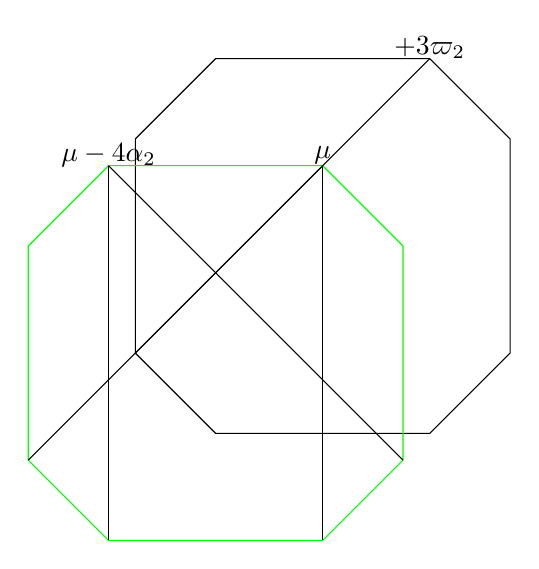
\begin{tikzpicture}[x=0.17cm,y=0.17cm]
\draw[black] (8,14) -- (-8,14) -- (-14,8) -- (-14,-8) -- (-8,-14) -- (8,-14) -- (14,-8) -- (14,8) -- cycle;
\draw[green] (-22,-16) -- (-22,0) -- (-16,6) -- (0,6) -- (6,0) -- (6,-16) -- (0,-22) -- (-16,-22) -- cycle;
\draw  (0,6)-- (-22,-16);
\draw  (0,6)-- (0,-22);
\draw  (-16,6)-- (-16,-22);
\draw  (-16,6)-- (6,-16);
\draw  (-14,-8)-- (8,14);
\node at (8,14.8) {$\lam+3\varpi_2$};
\node at (0,6.8) {$\mu$};
\node at (-16,6.8) {$\mu-4\alpha_2$};
\end{tikzpicture}
\end{center}
\caption{We have $\mu-4\alpha_2\not \leq \lam+3\varpi_2$ and the NS staircase $(e_1,e_2)$ from \Cref{fig:staircase} cannot be extended.}
\label{staircasemax}
\end{figure}

\end{example}

\begin{lemma}\label{staircaseunique}
There exists at most one non-empty NS-staircase over $(\mu,\lam)$.
\end{lemma}
\begin{proof}
Assume that the there are two non-empty NS-staircases of the form $\mu\raw \mu-(n+i)\alpha\in E^N(\lam+i\varpi_2)$ and $\mu\raw \mu-(n'+i)\beta\in E^N(\lam+i\varpi_2)$. Now, if $\mu_1> 0$, by \Cref{mu1>0nonswap2} we have $\alpha=\beta=\alpha_2$ and if $\mu_1<0$ we have $\alpha=\beta=\alpha_{12}$, so in particular $\alpha=\beta$.

We can assume $n'<n$. Since $\mu \raw \mu - n\alpha\in E^S(\lam)$, by \Cref{corcon}.1), we have that $\mu\raw \mu -n\alpha\in E^S(\lam+\varpi_2)$. With this and  \Cref{corcon}.2), we get $(\mu\raw \mu -(n'+1)\alpha)\in E^S(\lam+\varpi_2)$. Our second NS-staircase must therefore be empty. 
\end{proof}





\begin{lemma}\label{ifN=0thenD=0}
If $\calN_m(\mu,\lam)=0$ and $\mu <t_{m}\mu\leq \lam$, then also $\affD_m(\mu,\lam)=0$.
\end{lemma}
\begin{proof}
Assume that $\mu_1>0$.
If $\mu\raw t_k\mu\in E^S(\lam)$ for $k\leq m$, then also $\mu \raw t_k\mu \in E^S(\lam+\varpi_2)$ by \Cref{corcon}. If $t_k\mu\not \leq \lam$ and $(\mu\raw t_k\mu)\in E^N(\lam+\varpi_2)$, then $t_k=s_{K\delta-\alpha_2^\vee}$. But this cannot happen by \Cref{smallerissmaller}.

The case $\mu_1<0$ is symmetric.
\end{proof}

\begin{proposition}\label{Dcount}
 If $\mu_1>0$ we have
	\[ \affD_\infty(\mu,\lambda)=
	\begin{cases}
	\max(0,\min(\lam_1,\mu_1)-1) &\begin{array}{l}\text{if }-\lam_2\leq \mu_2\leq \lam_2 \\\text{ and }\mu_2\not\equiv\lam_2 \pmod{2};\end{array}\\
\max(0,\min(\mu_1,\lam_1)+\lam_2+\mu_2) &\begin{array}{l}\text{if } \mu_2<-\lam_2;\end{array}\\
0 &\begin{array}{l}\text{otherwise}.\end{array}
\end{cases}
\]
\end{proposition}
\begin{proof}
 Let $(e_i)_{1\leq i \leq a}=(\mu\raw v_{M+i}\mu)_{1 \leq i \leq a}$ be a non-empty maximal $NS$-staircase over $(\mu,\lam)$ with $M\geq -\mu_2$.

Assume first $\mu_1\geq \lam_1$. We have $e_1=(\mu\raw v_{M+1}\mu)\in E^N(\lam+\varpi_2)$, so by \Cref{mu1geqlam1} we get $\mu_2<-\lam_2$ or $M+1> \frc{\lam_2+1-\mu_2}$. We have either $v_M\mu=\mu$  or $e_0=(\mu\raw v_M\mu)\in E^S(\lam)$.
In the first case we get $-M=\mu_2$. In the second case we have $\mu_2\geq -\lam_2+1$, $M\leq \frc{\lam_2-\mu_2}$ and $M+1> \frc{\lam_2+1-\mu_2}$, so the only possibility is \[M=\frc{\lam_2-\mu_2}=\frc{\lam_2-\mu_2+1},\]
which also implies $\lam_2\not\equiv \mu_2 \pmod{2}$.

Assume further that $\mu_2<-\lam_2$.
From the discussion above we must have $M=-\mu_2$. It is easy to check that for any $k\geq 1$ we have $e_k\in E^N(\lam+k\varpi_2)$ if  $v_{M+k}\mu \leq \lam+k\varpi_2$ and that \[v_{M+k}\mu \leq \lam+k\varpi_2\iff \frf{\lam_1+\lam_2+\mu_2-k} \geq 0\]
so we get $\affD_{\infty}(\mu,\lam)=\max(0,\lam_1+\lam_2+\mu_2)$.

Assume now $\mu_2\geq -\lam_2$. If $\lam_2\not\equiv \mu_2 \pmod{2}$ then $\affD_\infty(\mu,\lam)=0$. If $\lam_2\not\equiv \mu_2 \pmod{2}$ we must have $M=\frc{\lam_2-\mu_2}$.
Since $v_M\mu\leq \lam$, from \eqref{eqtu} we get
%\[M\leq \frac{\lam_1-\mu_1}{2}-\mu_2+\min(\frf{\lam_2+\mu_1+\mu_2},\lam_2),\]
%so in particular 
\[ \frc{\lam_2-\mu_2}\leq \frf{\lam_1+\lam_2-\mu_2},\]
so this is possible only if $\lam_1 > 0$.
It easy to check that for any $k\geq 1$ if $v_{M+k}\mu \leq \lam + k\varpi_2$, then also $(\mu\raw v_{M+k}(\mu))\in E^N(\lam+k\varpi_2)$. Moreover, from \eqref{eqtu} $v_{M+k}\leq \lam+k\varpi_2$ we see that is equivalent to
%\[ \frc{\lam_2-\mu_2}\leq \frac{\lam_1-\mu_1}{2}+\frf{\lam_2+\mu_1-\mu_2+k}\]
\[\frc{\lam_2-\mu_2}\leq \frf{\lam_1+\lam_2-\mu_2-k}\]
which is true if and only if $k\leq \lam_1-1$. Hence $\affD_\infty(\mu,\lam)=\max(0,\lam_1-1)$.

The proof in the case  $0<\mu_1 < \lam_1$ is similar.
Since $e_1\in E^N(\lam+\varpi_2)$ we have $M+1>\frac{\lam_1-\mu_1}{2}+\max(-\mu_2,\frc{\lam_2-\mu_2+1})$. We have either $v_M\mu=\mu$ or $(\mu\raw v_M\mu)\in E^S(\lam)$. However, the first case is not possible because 
\[M+1=-\mu_2+1\leq \frac{\lam_1-\mu_1}{2}+\max(-\mu_2,\frc{\lam_2-\mu_2+1}).\]
In the second case, we have $M\leq \frac{\lam_1-\mu_1}{2}+\max(-\mu_2,\frc{\lam_2-\mu_2})$, which forces 
\begin{equation}\label{maxequality}
\max(-\mu_2,\frc{\lam_2-\mu_2})=(-\mu_2,\frc{\lam_2-\mu_2+1})
\end{equation}
 and $M=\frac{\lam_1-\mu_1}{2}+\max(-\mu_2,\frc{\lam_2-\mu_2}).$
The equality in \eqref{maxequality} can only occur if $\mu_2< -\lam_2$ or if $\mu_2\geq -\lam_2$ and $\lam_2\not \equiv \mu_2 \pmod{2}$.

Assume now $\mu_2<-\lam_2$. Then $M=\frac{\lam_1-\mu_1}{2}-\mu_2$. It is easy to check that for any $k\geq 1$ we have $e_k\in E^N(\lam+k\varpi_2)$ if  $v_{M+k}\mu \leq \lam+k\varpi_2$ and that \[v_{M+k}\mu \leq \lam+k\varpi_2\iff \frf{\mu_1+\lam_2+\mu_2-k} \geq 0\]
so we get $\affD_{\infty}(\mu,\lam)=\max(0,\mu_1+\lam_2+\mu_2)$.

Finally assume $\mu_2\geq -\lam_2$. If $\lam_2\not\equiv \mu_2 \pmod{2}$ then $\affD_\infty(\mu,\lam)=0$. If $\lam_2\not\equiv \mu_2 \pmod{2}$ we must have $M=\frac{\lam_1-\mu_1}{2}+\frc{\lam_2-\mu_2}$.
%\[M\leq \frac{\lam_1-\mu_1}{2}-\mu_2+\min(\frf{\lam_2+\mu_1+\mu_2},\lam_2),\]
%so in particular 
It easy to check that for any $k\geq 1$ if $v_{M+k}\mu \leq \lam + k\varpi_2$, then also $(\mu\raw v_{M+k}(\mu))\in E^N(\lam+k\varpi_2)$. Moreover, from \eqref{eqtu} $v_{M+k}\leq \lam+k\varpi_2$ we see that is equivalent to $k+1\leq \mu_1$.
 Hence $\affD_\infty(\mu,\lam)=\max(0,\mu_1-1)$.
\end{proof}

\begin{corollary}\label{Dinf<0}
If $\mu_1<0$ we have 
\begin{align*}\affD_\infty(\mu,\lambda) =\begin{cases}
	\max(0,\min(\lam_1,-\mu_1)-1) &\begin{array}{l}
 \text{if }-\lam_2\leq \mu_1+\mu_2\leq \lam_2 \\\text{and } \mu_1+\mu_2\not\equiv\lam_2 \;(\mathrm{mod }\;2);\end{array}\\
\max(0,\min(-\mu_1,\lam_1)+\lam_2+\mu_1+\mu_2) \hspace{-10pt}&\begin{array}{l}\text{if } \mu_1+\mu_2<-\lam_2;\end{array}\\
0 &\begin{array}{l}\text{otherwise}.\end{array}\end{cases}\end{align*}
\end{corollary}
\begin{proof}
    This immediately follows from \Cref{Dcount}, since by symmetry (cf. \Cref{12notswap}) we have $\affD_{\infty}(\mu,\lam)=\affD_{\infty}(s_1(\mu),\lam)$.
\end{proof}


Suppose than $T\in \calA(\lamk)\subset \calP(\lam)$.
In our applications in \Cref{sec:swapping}, we are only interested in NS staircase over $(\wt(T),\lamk)$ that live inside the preatom $\calP(\lam)$. In other words, we truncate our NS staircases $(e_i)_{1\leq i\leq a}$ so that $a\leq k$. 

The following quantity measures the longest possible truncated NS staircase over $(\mu,\lamk)$ in a preatom of highest weight $\lambda$.
\begin{definition}
\label{truncatedns}
Assume that $k\geq 0$ and $\mu \leq \lam-k\varpi_2$. Then, for any $m\in \bbN\cup \{\infty\}$ we define
\[ \calD_m(\mu,\lam,k):=\min(k,\affD_m(\mu,\lam-k\varpi_2)).\]
\end{definition}

